\chapter{作为一个整体的前额叶皮层:从当前环境和事件中产生目标} \label{chap:chap8}

% 晓来不戴催征鼓,红日方升已奋楫
\section{概述}

颗粒状前额叶皮层位于三个信息处理层次的顶部:
一个用于当前上下文,
另一个用于目标,
第三个用于行为结果。
作为上下文层次的顶点,前额叶皮层整合了空间和非空间视觉、触觉和内脏感觉、听觉、味觉和嗅觉的皮层输入,以及来自海马体的输入。
作为目标层次的顶点,前额叶皮层代表行动的目标,包括具体和抽象目标的序列、集合和类别,它可以通过与运动前皮层的联系来影响他们的活跃度。
作为结果层次的顶点,它代表了特定食物和液体的所有感官维度,并通过与杏仁核的联系,根据当前的生物需求更新了它们的动机评估。
通过整合这三个层次,类人猿前额叶皮层可以产生适合当前环境和当前需求的目标。
作为对类人猿进化过程中面临的觅食问题的一种特殊适应,它们可以学会在单一事件的基础上产生目标,从而减少危险或无效的觅食选择。
类人猿灵长类动物比它们的祖先更快地解决新的觅食问题,因为它们新进化的前额叶皮层实现了一个快速、通用的学习系统,这增强了动物历史早期进化的祖先强化学习机制。



\section{介绍}
\par

前面的五章把前额叶皮层拆开了,现在是时候把它重新组装起来了。
第~\ref{chap:chap3}~章和第~\ref{chap:chap4}~章分别讨论了内侧前额叶皮层和眶额皮层。
例如,我们认为,关于当前生物需求的信息通过与杏仁核的连接到达眶额皮层,并且海马体向内皮层提供关于导航和其他涉及动作的事件的信息。
第~\ref{chap:chap5}~章从搜索和注意力的角度解释了尾侧前额叶皮层的功能,通过与背侧和腹侧视觉流的连接来实现。
第~\ref{chap:chap6}~章提出,关于空间、时间和序列的信息从后顶叶皮层到达背侧前额叶皮层,并有助于基于这些内容的上下文进行选择。
第~\ref{chap:chap7}~章说,关于视觉和听觉信号的信息从颞叶皮层到达腹侧前额叶皮层,并在其他情境的基础上做出选择。
\par


这种讨论前额叶皮层的方式可能会造成这样一种印象,即它是作为五个独立的区域运作的。
但前额叶皮层是一个整体,它能这样做是因为它的内在联系允许它整合通过不同通路到达的信息。
因此,灵长类动物的前额叶皮层可以根据对结果和整体环境的总体预测来生成目标。
前额叶皮层的贡献超出了这种深远的整合,但以这种方式将信息聚集在一起的能力是其基本功能的基础之一。
\par


由于前额叶皮层作为一个整体发挥作用,我们需要一个全面的理论,而第~\ref{chap:chap1}~章提出了这样一个理论的两个要求:
展示前额叶皮层能做大脑其他部分不能做的事情,并解释为什么它的连接使它能够以这种方式发挥作用。
像以前一样,我们从联系开始。



\section{联系}
\par
第~\ref{chap:chap3}-\ref{chap:chap7}~章每个章节都有一个部分强调了前额叶皮层的一个部分的连接。
我们在这里总结总体模式。



\subsection{皮层和杏仁核}

\begin{enumerate}
\item 颗粒状前额叶皮层接收来自视觉、听觉、体感、嗅觉、味觉、嗅觉和内脏皮层的信息。
因此,灵长类动物的前额叶皮层有相对直接的来自距离感受器的输入,如视觉和听觉感受器,以及传递特定行为结果的输入,如食物和液体的味觉、嗅觉、视觉和感觉。
因此,灵长类动物的前额叶皮层对特定的行为结果有一个强大的、高维的表征,特别是包括它们的视觉属性。
它还具有复杂的视觉和听觉表征,可以指导觅食或社会选择。
视觉标志反映了灵长类动物的一些进化进步,如中央凹和三色视觉。
其他哺乳动物的前额叶皮层和灵长类动物新皮层的其他部分至少缺乏这些特性中的一些。

\item 前额叶皮层还接收来自海马体和海马复合体其他部分的直接和间接输入。
海马体、下托和内嗅皮层都与内侧前额叶皮层有直接联系。
海马体在导航和事件记忆中发挥作用,尤其是对于嵌入其空间和时间背景中的事件和对象。
与前额叶皮层一样,海马复合体接收来自所有感觉模式的输入,并与杏仁核紧密相连,传达行为的某些方面结果。
但是,尽管前额叶皮层通过运动前区域有直接输出,但海马体对这些区域的直接访问较少,缺乏前额叶皮层所具有的那种内在联系,也没有前额叶皮层所拥有的那种直接、特定的结果信息(详情见第~\ref{chap:chap4}~章)。


\item 杏仁核与前额叶皮层的许多部分有着紧密的联系(见图~\ref{fig:3_3})。后顶叶皮层等区域几乎没有这种联系。
一些运动前区与杏仁核有联系,但它们很稀疏\cite{avendan1983evidence}。
前额叶皮层和杏仁核的连接在根据动物的当前状态更新行为结果的动机评估中发挥作用。
因此,前额叶皮层能够以后顶叶和运动前皮层所没有的方式代表更新的评估值。

\item 前额叶皮层直接或间接投射到内侧和外侧前运动区域,从而可以为这些区域提供运动目标。
前运动皮层的嘴侧部分与前额叶皮层有着广泛的联系,但尾侧部分也从前额叶皮层获得信息,尽管不那么直接。
这些连接在很大程度上排除了腿部和脚部的运动表示。
与后肢表现相反,前肢的特化表现在背侧前运动皮层的喙部\cite{tachibana2004input}、腹侧前运动皮层\cite{he1993topographic}、前扣带回皮层\cite{luppino1991multiple}和头侧扣带运动区\cite{he1995topographic}。
正如第~\ref{chap:chap2}~章所解释的,这种前肢偏向反映了灵长类动物以后肢为主的运动形式,这使手可以自由发挥其他功能。
通过与运动前区域的连接,前额叶皮层在伸手、抓握和操纵方面发挥着优先作用,而不是运动能力。
这些联系促进了目标的实现,例如抓住物体或到达某个地方。


\item 前额叶皮层也有控制注意力和搜索功能的连接,包括对应于显性注意力的眼球运动(详情第~\ref{chap:chap5}~章)。
例如,尾侧前额叶皮层既有到脑干动眼神经核的直接投射,也有通过上丘和基底神经节的间接投射。
第~\ref{chap:chap2}~章指出,灵长类动物的大多数颗粒状前额叶皮层具有强烈的皮层顶盖投射\cite{leichnetz1981prefrontal}。
前额叶皮层还向顶叶和颞叶发送投射,介导对背侧和腹侧视觉流以及其他感觉模式的自上而下的注意力。


\item 灵长类动物前额叶皮层的各个部分之间有着广泛的联系。这些预测已在其他地方详细记录\cite{barbas1988anatomic,carmichael1995sensory,barbas1999medial,petrides1999dorsolateral,petrides2002association,price1999delineating}。
来自前额叶皮层外部的任何输入都可以在两个突触内到达前额叶皮层的任何部分\cite{averbeck2008statistical}。
前额叶皮层不仅接收大量输入,而且无论信息最初到达哪里,它都可以快速组合这些输入。
\end{enumerate}
\par


除了与皮层的其他部分和杏仁核的连接外,灵长类动物的前额叶皮层还与屏状核、基底神经节、丘脑、中脑中的多巴胺能神经元和小脑有连接。
接下来的五节依次介绍这些内容。



\subsection{屏状核}
\par

屏状核与前额叶皮层有相互联系\cite{tanne2002projections},也通过丘脑的\textit{背内侧核}投射到它\cite{erickson2004subcortical}。
它与皮层的其余部分也有类似的联系。
来自几个皮层区域的投影汇聚在一个特定的屏状核区,每个屏状核区都连接到额叶的几个部分,包括前额叶皮层\cite{tanne2002projections}。
这种连接模式表明屏状核可能达到了一定程度的整合。
然而,它似乎缺乏前额叶皮层特有的广泛的内在联系。



\subsection{基底神经节}
\par

与大多数大脑皮层一样,前额叶皮层向基底神经节发送一个沉重的投射,靶向其输入结构纹状体。
尽管大部分(如果不是全部的话)大脑皮层都有大量的输入,但基底神经节的输出似乎集中在额叶,尽管一些输出也流向了后顶叶\cite{clower2005basal}和颞叶皮层\cite{middleton1996temporal}。
这种组织表明,前额叶皮层和基底神经节之间的联系也可能有助于其在整合信息方面的作用。
\par


然而,它对这种整合的贡献方式仍然存在争议。
基底神经节缺乏能够整合其各个部分信息的远距离内在联系。主流观点强调皮层-基底神经节环的平行组装,重叠最小\cite{alexander1991basal,nakano2000neural}。
图~\ref{fig:8_1}~描述了其中一些环,包括一个前运动区(辅助运动区)和几个前额叶区。
Middleton\cite{middleton2000basal}得出结论,总的来说,涉及前额叶皮层的环在解剖学上与涉及运动前区域的环不同。
如果这是真的,基底神经节组织的这一特征表明大多数整合发生在皮层水平,尽管纹状体和黑质纹状体投射的某些方面可以提供一些整合能力。
他们这样做可能是因为一种叫做向上螺旋的组织特性\cite{haber2000striatonigrostriatal}。
黑质纹状体突起不仅回到为黑质的特定部分提供纹状体的环,而且还回到相邻的环。



\subsection{丘脑}
\par

前额叶皮层和所有其他皮层区域一样,与丘脑有相互联系。
它的主要丘脑连接是与\textit{背内侧核}。
例如,\textit{背内侧核}的多形部分接收来自上丘的输入\cite{russchen1987afferent,erickson2004subcortical},并投射到尾侧前额叶皮层,而后者又投射到上丘脑\cite{fries1984cortical}。
这些联系有助于引起明显和隐蔽的注意(第~\ref{chap:chap5}~章)。
\par


同样,内侧大细胞\textit{背内侧核}投射到眶额皮层\cite{ray1993organization},并接收来自杏仁核的输入\cite{russchen1987afferent}。
所以研究人员一点过也不惊讶于\textit{背内侧}大细胞分裂的病变具有与眶额皮层或杏仁核病变相似的影响\cite{mitchell2007neurotoxic}(见第~\ref{chap:chap4}~章)。
Izquierdo\cite{izquierdo2010functional}已经证明了在强化剂退化任务中,大细胞\textit{背内侧核}和眶额皮层的功能相互作用。


\begin{figure} 
	\centering
	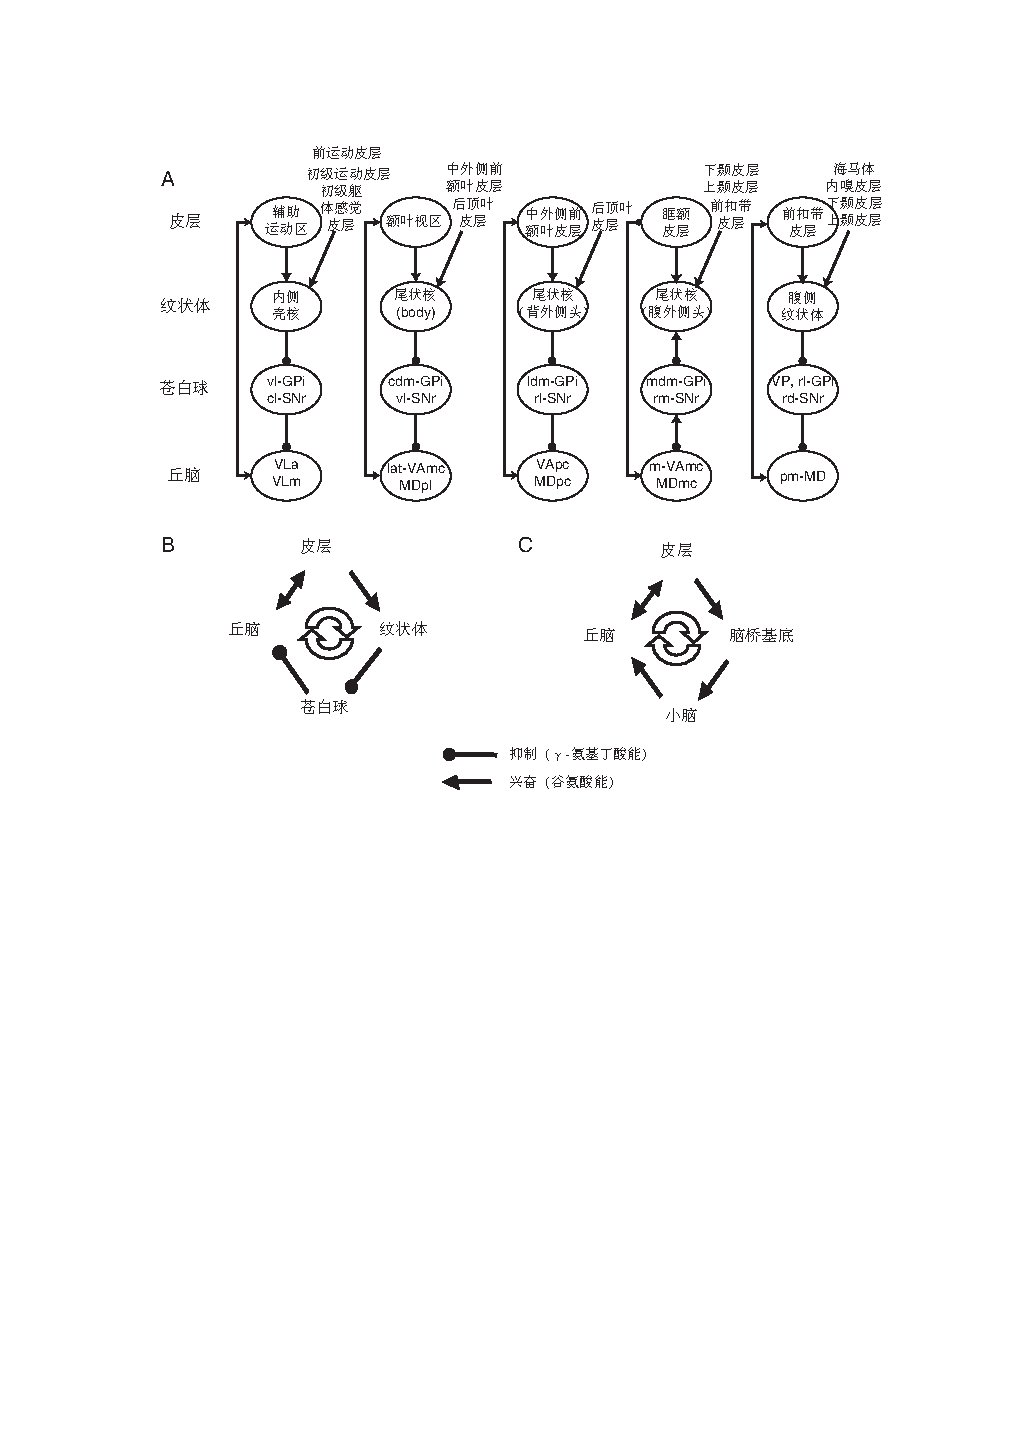
\includegraphics[width=0.72\linewidth]{chap8/fig_8_1}
	\caption{(A)选定的皮层-基底神经节环\cite{alexander1986parallel}。
	皮层区和皮层下核的缩写:AC,前扣带皮层; Caud,尾状核; 耳鼻喉科,内嗅皮层; FEF,额叶视区; GPi,苍白球内段; 海马,海马; IT,下颞叶皮层; M1,初级运动皮层; MD,丘脑内侧核; 中背侧 PF,中外侧 PF 皮层; 中壳核,不包括喙壳核和尾壳核的壳核; PM,前运动皮层; PP,后顶叶皮层; S1,初级体感皮层;SNr,黑质网状核; ST,颞上皮层; VA,丘脑腹前核; VL,丘脑腹外侧核; VP,腹侧苍白球; VS,腹侧纹状体。 细分缩写:a,前; cdm,尾内侧; cl,尾外侧; dl,背外侧; 纬度,横向; ldm,后内侧; m,内侧; mc,大细胞; mdm,中背内侧; 个人计算机,细细胞; pl,平行板层; pm,后内侧; rd,吻背侧; rl,头外侧; rm,吻内侧; vl,腹外侧。
	(B)皮层-基底神经节环路的总体连接方案。 
	(C)皮层-小脑环路的总体连接方案\cite{shadmehr2004computational}。\label{fig:8_1}}
\end{figure}





\subsection{多巴胺能中脑}
\par

前额叶皮层的一些输入来自中脑的多巴胺能神经元。
正如第~\ref{chap:chap3}~章所提到的,这些细胞提供了奖励预测误差信号\cite{schultz1998predictive}。
关于这种信号的大多数理论工作都集中在它作为纹状体教学信号的作用上,但其中一些细胞也直接投射到前额叶皮层和其他区域\cite{gaspar1992topography},它们可以在皮层和纹状体水平上促进学习\cite{miller2007rules}。



\subsection{小脑}
\par

就像皮层和基底神经节之间存在的回路一样,皮层和小脑在解剖学回路中相互连接。
这些环涉及脑桥基底核和丘脑\cite{houk1995distributed}。
在前额叶区域中,尾侧前额叶皮层和背侧前额叶皮层向桥基底核发送最大的投射,只有少量的桥皮层投射来自腹侧或眶额皮层\cite{schmahmann1997anatomic,glickstein2008cerebellum}。
Middleton\cite{middleton1998cerebellar,middleton2001cerebellar}已经表明,皮层和小脑之间的环路包括中外侧前额叶皮层(区域46)和背内侧前额叶皮层(区域9)。



\subsection{摘要}
\par

前额叶皮层连接的简要草图从第~\ref{chap:chap3}-\ref{chap:chap7}~章中提取了一些关键点,这些关键点涉及每个区域的连接。
我们强调前额叶皮层中信息的汇聚和整合,就像我们之前的许多其他结构一样。
但第~\ref{chap:chap3}~章至第~\ref{chap:chap7}~章也具体说明了灵长类动物前额叶皮层如何做大脑其他部分无法做的事情。
这些其他结构中的一些缺乏足够的内在连接,另一些缺乏关于特定结果更新估值的输入,而其他的则无法直接进入运动前皮层。
\par


前额叶皮层接收各种各样的输入,其内在联系可以快速整合,并对动作产生直接影响。
第~\ref{chap:chap3}~章至第~\ref{chap:chap7}~章提供了证据,证明其细胞负责编码多种信息之间的连词。
下一节将这些特性放在信息处理层次结构的上下文中。



\section{层次结构}
\par

Fuster\cite{fuster2000executive}长期以来一直认为,我们应该从层次结构的角度来看待颗粒前额叶皮层。
在他看来,颗粒前额叶皮层形成了从感知到行动的最高联系:用他的术语来说,就是感知-行动循环。
然而,要理解颗粒前额叶皮层,我们需要的不仅仅是层次概念以及感觉输入和运动输出之间的联系。
我们需要知道当这些联系涉及颗粒前额叶皮层时,它们之间的区别。
Fuster指出,它们在层次等级上有所不同。
我们同意这种观点,但要将这一想法转化为前额叶皮层的成功理论则需要更加精确。
\par


为了达到这一精度,我们需要解释我们所说的层次制度是什么意思。
从某种意义上说,与较低的成分相比,较高的成分位于离感觉输入或运动输出更远的层次中。
从另一个意义上说,更高的级别更抽象地表示信息。
从第三种意义上来说,层次结构的更高层次表示具有更高维度的信息,即具有更高程度的特征连接。
\par


我们认识到,第二种意义和第三种意义在某些方面存在冲突。
正如这个词所暗示的那样,抽象涉及提取不同表征的共同特征,而更高维度则需要通过添加特征来区分表征。
尽管如此,我们认为抽象和高维表示在这里讨论的层次结构中都很高。
例如,“猫”的抽象概念包括豹猫、美洲虎和老虎,但并不具备任何特定猫种的所有特征,当然也不具备邻居的虎斑猫。
从这个意义上说,抽象在层次上是很高的,尽管它们需要更少的特性。
但同样真实的是,将许多特征合成为一个逐渐更具体的表示,反映了沿着等级制度的上升,正如通常所解释的那样。
基于皮层细胞及其末端的层流分布的前馈和反馈连接模式有时反映了这种层次结构\cite{rockland2000feedback}。



\subsection{上下文层次结构}
\par
前额叶皮层比其他区域离初级感觉区域更远,它接收来自所有初级感觉区域的汇总输入。
Jones首次认识到皮层组织的这一特征,他们的结论是基于连接解剖学的研究\cite{jones1970anatomical}。
例如,他们指出了腹侧视觉流,它处理有关颜色、形状和视觉纹理的信息。
它在颞叶的喙部达到顶峰,包括TE区和嗅周皮层区域。
由于TE区\cite{webster1994connections}和嗅周皮层\cite{petrides2002association}都向颗粒状前额叶皮层发送投影,所以前额叶皮层可以被视为位于视觉处理层次的顶点\cite{young1992objective}。
\par


类似的结论适用于听觉输入\cite{romanski2009primate}和触觉输入\cite{jones1970anatomical}。
味觉和内脏输入通常平行于体感通路,并遵循类似的组织原则。
嗅觉系统是一种特殊情况,但这些输入也从初级嗅觉区域梨状皮层通过无颗粒前额叶皮层传递到颗粒前额叶皮层(第~\ref{chap:chap4}~章)。
因此,颗粒前额叶皮层位于信息处理层次结构的顶部,该层次结构集成了所有感觉模式来表示当前的行为背景。
前额叶皮层还可以整合来自海马体和杏仁核的信息,以及上一节提到的其他结构,如基底神经节和小脑。
\par


上下文层次结构可以从其连接中识别出来,但其他方法也揭示了同样的东西。在猕猴中,基底树突树的大小和树突棘的数量从V1到V2、V4、TEO和TE等区域一直在增加,并且这种趋势持续到前额叶皮层\cite{elston2007specialization}。
这种层次结构在额极皮层达到顶峰。
树突发育的增加可能支持神经整合能力的增强。
\par


正如第~\ref{chap:chap4}~章所指出的,前额叶皮层中的上下文层次扩展了腹侧视觉流开始的特征连接\cite{murray2007visual}。
在视觉层次结构的越来越高的层次上,更多的特征进入这些连接。
在颗粒前额叶皮层中,来自无颗粒前额叶皮层的输入与来自颞叶和顶叶皮层的输入汇合,以建立更高阶的多模式连接,包括视觉、听觉、触觉、味觉、嗅觉和内脏特征(见图~\ref{fig:fig_4_3})。
\par


第~\ref{chap:chap2}~章指出,颞下区TE与颗粒状前额叶皮层一样,是在灵长类动物中进化而来的。
这个想法有一个重要的含义。
灵长类动物的进化既不是嗅周皮层的高级特征连接,也不是纹状体皮层(V1)和其他枕叶区域的低级元素表示。
V1和嗅周皮层出现在所有哺乳动物中,因此很可能在早期哺乳动物中进化。
灵长类动物的颞下皮层(TE和TEO区域)进化较晚,这些区域提供中等水平的视觉处理。
它的细胞既不代表整个物体,也不代表低级的基本特征。
颞下皮层和嗅周皮层都向除了尾侧前额叶皮层以外的颗粒前额叶皮层发送输入,但枕叶区域不发送输入(第~\ref{chap:chap5}~章)。
因此,大多数颗粒状前额叶皮层接收来自视觉层次的中间和更高层次的输入,而不是来自较低层次的输入。
\par


第~\ref{chap:chap2}~章和第~\ref{chap:chap7}~章指出了资源视觉标志的重要性。
这些线索也介于物体和简单的视觉特征之间。
此外,颞下皮层处理有关面部的信息\cite{baylis1987functional,tanaka1991coding},这些信息也提供“迹象”或“线索”。
声学呼叫也起到信号的作用,颞上皮层的细胞编码特定的呼叫,比如打招呼\cite{rauschecker1995processing}。
通过与视觉对象的类比,颞叶皮层的声学表征有时被解释为“对象”,但通过与中级视觉信号的类比,将其视为信号可能更有用。
因此,灵长类动物的大脑已经进化为将听觉和视觉线索都视为信号,而且似乎是通过在颞叶中创建一个介于物体和基本特征之间的中间水平的特征连接来做到这一点的。
\par


第~\ref{chap:chap7}~章解释了颗粒状前额叶皮层利用手势作为目标生成的背景,前一段提到了颞下皮层的面部响应细胞。
考虑到颞下皮层与腹侧前额叶皮层和眶额皮层之间的联系,在这些额叶区域出现类似的响应并不奇怪。
ÖScalaidhe等人\cite{o1999face}研究了腹侧前额叶皮层(12/47区)、背侧前额叶皮层(9区和46区)和尾侧前额叶皮层(8区)的细胞活性。
他们发现,在接受颞下皮层输入的区域,即腹侧前额叶皮层,会有选择性地对人脸做出响应,但在其他区域没有。
面部细胞与对物体和彩色图案有响应的细胞混合在一起。
重要的是,这些特性都不依赖于实验室任务的事先训练。
\par


类似的响应发生在眶额皮层。
Rolls等人\cite{rolls2006face}描述了那里对人脸有选择性响应的细胞。
其中一些细胞对人脸识别有响应,另一些细胞对面部表情有响应,还有一些细胞对移动的头部有响应,但对静止的头部没有响应。
其中一些细胞对不同的视角表现出选择性,但另一些细胞的响应是不变的。
\par


所有这些细胞都可以在社交互动中发挥重要作用,它们都有助于上下文层次。
面部表情和面部特征为社会选择提供了重要标志,就像其他视觉标志为觅食选择提供的一样。
声学信号在社交和觅食选择中也起着至关重要的作用。
与觅食选择一样,社会选择涉及基于当前环境和当前生物需求产生目标。
当然,动机往往各不相同。
\par


一些发现指出了整合视觉和听觉信号的重要性,颗粒状前额叶皮层处于执行这一功能的良好位置。
颞上沟下岸的细胞对面部做出响应,并且在面部和叫声的同时出现的情况下表现出增强的活跃度\cite{barraclough2005integration}。
这些区域与颗粒状前额叶皮层有联系,因此腹侧前额叶皮层中的细胞表现出类似的作用也就不足为奇了\cite{sugihara2006integration}。
\par


视觉和听觉整合的另一个例子涉及条件学习,如配对联想学习任务(第~ \ref{chap:chap7}~章)。
Fuster等人\cite{fuster2000executive}训练猴子在一个音调下选择红色刺激,在另一个音调上选择绿色刺激。
他们从尾侧前额叶皮层(8B区)进行了记录,发现了对其中一种音调以及与该特定音调相关的颜色有选择性响应的细胞。
这个属性对应于第~\ref{chap:chap7}~章提到的视觉-视觉关联的配对编码。
模态内和跨模态的结果都反映了延迟区间的积分,这是我们稍后讨论的主题。
\par


额叶整合的最后一个例子涉及不同类型的视觉信息,如形状和位置,分别是腹侧和背侧视觉流的区域。
前额叶皮层连接到两个流(第~\ref{chap:chap5} - \ref{chap:chap7} ~章),但Wilson等人\cite{wilson1993dissociation}认为,它们的信号可能在颗粒状前额叶皮层中保持分离。
然而,Rao等人\cite{rao1997integration}在中外侧前额叶皮层和腹侧前额叶皮层中发现了编码记忆形状和记忆位置的单细胞。
因此,前额叶皮层的内在连接将首先到达其不同部分的信号汇集在一起,就像来自背侧和腹侧流的输入一样(第~\ref{chap:chap5}~章和第~\ref{chap:chap7}~章)。
\par

这些上下文整合的例子涉及感官信息,但要完全指定当前的上下文,类人灵长类动物还必须考虑特定时间和地点的目标、行动和结果。
前额叶皮层与海马体的连接可能提供了上下文层次结构的一些方面(第~\ref{chap:chap3}~章)。
除了感官环境外,导航历史和事件信息都在觅食选择中发挥着至关重要的作用。
除了位置和对象标识外,顺序和时间在事件处理中也起着重要作用。
例如,第~\ref{chap:chap6}~章解释了中外侧前额叶皮层的细胞编码顺序-画面连接\cite{warden2007representation}。
同样,中外侧前额叶皮层和尾侧前额叶皮层中的细胞编码顺序-持续时间\cite{tsujimoto2009monkey}和顺序-距离连接(Genovecio等人,2011年)。
其他前额叶皮层细胞本身也编码刺激顺序\cite{ninokura2003representation,ninokura2004integration}。
据推测,这些细胞为编码连词的细胞提供了输入。
\par


总之,颗粒状前额叶皮层整合了来自所有感觉模式的感觉输入。
它在模态内部和模态之间都是这样做的,它对当前刺激和最近发生的刺激都是这样,对整个物体和位于基本特征和整个物体之间的特征连词都是如此,我们称之为符号。
它将这些多模式输入与有关事件的信息集成在一起,包括事件的顺序、地点和时间,以作为上下文层次结构的最高级别。其他皮层区具有某些财产,但没有其他皮层区具备所有这些属性,以及直接进入运动前区。



\subsection{目标层级}
\par
正如前额叶皮层离初级感觉区相对较远一样,它也比初级体感皮层、运动前皮层(6区)和顶叶后皮层的嘴侧部分(5区)等区域离初级运动皮层更远。
这些额叶和顶叶区域都向初级运动皮层发出直接投射,但颗粒状前额叶皮层没有\cite{jones1970anatomical,lu1994interconnections}。
它们中的每一个也直接投射到脊髓,而颗粒状前额叶皮层缺乏这种投射\cite{murray1991contributions}。
直接进入初级运动皮层和脊髓的程度定义了一个层次。
因此,我们可以将颗粒状前额叶皮层描述为位于运动层次的顶部。
或者,由于运动系统产生动作,我们可以称之为Fuster\cite{fuster1988prefrontal}所说的动作层次。
相反,我们选择将前额叶皮层组织的这一方面称为目标层次。
我们这样做是因为我们认为颗粒状前额叶皮层是产生目标的,而不是像前几章所解释的那样认为是行动或运动。
然而,如果读者将目标层次结构视为目标-行动层次结构,我们也不会反对。
与后顶叶皮层一起,颗粒状前额叶皮层投射到运动前皮层,这一途径为前额叶皮层提供了对动作控制的最直接影响。
后顶叶皮层最大量地投射到背侧前运动皮层的尾部和\textit{辅助运动区},而颗粒状前额叶皮层最大量的投射到前运动皮层\cite{rizzolatti2001cortical,luppino2003prefrontal}。
运动前皮层的喙前部分反过来又与其尾部相连。
例如,前\textit{辅助运动区}投射到\textit{辅助运动区},\textit{辅助运动区}又将轴突直接发送到初级运动皮层\cite{luppino1993corticocortical}和脊髓\cite{murray1981organization}。
\textit{辅助运动区}前区和喙前运动区投射到前运动皮层的尾部,但不投射到脊髓\cite{he1995topographic}。
因此,额叶的目标层次在其较低水平上可以直接进入初级运动皮层和脊髓,而这种层次在较高水平上继续进入颗粒状前额叶皮层。
为了解释这种层次结构,我们从初级运动皮层开始。
图~\ref{fig:1_10}~显示,初级运动皮层(4区)的细胞在记忆引导的运动和可见线索引导的运动中具有相同的活动。
背侧前运动皮层和\textit{辅助运动区}的细胞通常分别表现出外部和“内部”引导的特异性。
Shima和Tanji(2000)在前\textit{辅助运动区}和\textit{辅助运动区}中进行了记录,并在这两个区域发现了编码特定作用序列的细胞。
然而,编码特定转变的细胞在\textit{辅助运动区}中比在前\textit{辅助运动区}中更常见。
相反,发出运动是序列中的第一个、第二个还是第三个信号的细胞在前\textit{辅助运动区}中比在\textit{辅助运动区}中更常见。
Shima和Tanji利用这些发现构建了一个产生运动序列的层次模型。
Cisek和Kalaska(2002)同样记录了背侧前运动皮层的头侧和尾侧部分。
当出现两个潜在靶点时,嘴侧部分的一些细胞编码两个靶点,但尾侧部分具有这种特性的细胞较少。
当猴子知道要瞄准哪个目标时,这两个部位的活动就指定了那个位置。
因此,从神经生理学和神经解剖学的角度来看,嘴侧前运动皮层和前\textit{辅助运动区}在运动层次上似乎比尾侧前运动皮层和\textit{辅助运动区}更高。
反过来,后一个区域似乎比初级运动皮层更高。
因此,这些区域形成了一个运动层次。
我们提出,颗粒状前额叶皮层将这种运动层次细化为目标层次。
例如,前\textit{辅助运动区}和\textit{辅助运动区}中的细胞编码给定的运动序列(Shima\&Tanji,2000),但颗粒状前额叶皮层中的细胞对序列的抽象结构进行编码(Shima等人,2007)。
正如第~\ref{chap:chap6}~章所解释的(见图~\ref{fig:6_12}),在序列之前具有活性的细胞中,超过一半的细胞编码了抽象结构,例如交替:拉、转、拉、转和推、拉、推、拉。
这种抽象并不是指特定的动作,而是指更高阶的表示。
有证据表明,运动前皮层将这些抽象概念转化为具体的运动计划(Hoshi,2008)。
除了抽象序列外,颗粒状前额叶皮层中的细胞还可以编码抽象的行为规则和策略,如匹配和不匹配规则(见图~\ref{fig:7_9})或“重复停留”和“改变-转移”策略(见图~\ref{fig:7_11})。
正如第~\ref{chap:chap7}~章所解释的,这些规则适用于任何刺激,它们产生了可供选择或避免的目标集或类别。
一组可能目标的抽象表示不同于特定目标的具体表示,例如单个对象或地点。
通过这种方式,颗粒状前额叶皮层中编码的表征有助于目标层次。
当与前额叶皮层中编码独立于实现目标的方法的细胞的发现一起考虑时,这一概念变得尤为重要(第~\ref{chap:chap6}~章和第~\ref{chap:chap7}~章)。
基于对这一点的讨论,读者可以理解目标和上下文层次结构有许多共同的财产。
对于这两种情况,颗粒状前额叶皮层位于解剖层次的顶端,该解剖层次包括其较低水平的其他大脑区域。
目标层次结构提供了几种方法,可以将当前上下文与具体动作的规范(根据电机命令)联系起来。
它通过指定用作动作目标的对象或位置,通过指定动作的一系列的抽象结构,或者通过指定生成要选择或避免的对象或地点的规则或策略来做到这一点。
在一系列层次上产生目标的能力,独立于实现目标的手段,代表了颗粒状前额叶皮层所赋予的一个重要优势。



结果层次结构

目标导致行动,行动导致结果。
与上下文一样,结果是由各种感觉模式产生的输入指定的。
然而,动物并没有进化出专门的奖励或结果受体。
然而,颗粒状前额叶皮层的连接使其能够以一种独特的方式分析结果(第~\ref{chap:chap4}~章)。
除了海马体之外,没有任何其他皮层区域具有如此多样化的输入阵列,也没有任何其他皮层区域能够有效地整合它们,同时相对直接地进入运动前皮层。
颗粒状前额叶皮层的结果层次结构既包括随着层次的上升而更大的特征收敛(见图~\ref{fig:fig_4_3}),也包括更大的抽象。
第~\ref{chap:chap4}~章回顾了特征收敛的证据。
眶额皮层中的细胞对视觉-味觉、视觉-嗅觉和味觉-嗅觉的结合做出响应(Rolls等人,1994年)。
这些组合对觅食选择具有明显的重要性:它们对构成结果的特定食物或液体进行编码。
除了编码食物和液体的物理财产外,前额叶皮层中的细胞还根据当前需求对其生物价值进行编码,正如贬值效应所揭示的那样(Izquierdo等人2004年)。
第 \ref{chap:chap4} 章还解释说,除了根据特定的食物和液体对结果进行编码外,作为结合许多特征的高维表征,眶额皮层的颗粒部分还根据抽象的“共同货币”对结果进行了编码,该货币代表一维的价值。
这两个层次在颗粒状前额叶皮层的功能中都起着重要作用。
当猴子在众多选择中选择追求哪个目标时,它们可以用抽象的估值来比较自己的选择;
当他们需要了解哪种选择导致了特定的结果时,他们可以将结果编码为许多刺激维度。
因此,结果层次结构的两个方面——增强的特异性和抽象性——都有助于颗粒状前额叶皮层的功能。
第 \ref{chap:chap4} 章提供的证据表明,颗粒状前额叶皮层的不同细分服从于结果层次的这两个方面:
横向眶额皮层编码特定的食物和液体,用于相互对比各种结果;
中间眶额皮层以“通用货币”对价值进行编码以进行比较。
当与杏仁核在更新结果估值中的作用相结合时(第 \ref{chap:chap4} 章),灵长类动物的前额叶皮层作为一个整体,提供了一种强大的机制,可以将特定结果的复杂表征与觅食选择相结合,包括那些基于“共同货币”抽象估值的表征。



总结

颗粒状前额叶皮层位于三个信息处理层次的顶端,其中包括处于较低水平的其他大脑结构。
上下文层次结构建立在感觉区的功能;目标层次阐述了运动区域的功能,以及内侧前额叶皮层的无颗粒部分;
并且结果层次建立在眶额皮层的无核部分上。
请注意,我们还没有讨论颗粒状前额叶皮层内的层次结构,下一章将对此进行讨论。
通过整合这三个层次,颗粒状前额叶皮层可以将上下文映射到目标和预测结果。
第 \ref{chap:chap3} 章展示了前额叶皮层是如何对目标层次做出贡献的;
第 \ref{chap:chap4} 章讨论了前额叶皮层对结果层次的贡献。
第 \ref{chap:chap5} 章通过整合对象和地点的目标和结果层次,指出前额叶皮层在寻找和关注目标方面的作用。
关于上下文层次,第 \ref{chap:chap6} 章讨论了从位置、顺序和时间上下文生成目标;
第 \ref{chap:chap7} 章涉及从视觉和听觉信号中产生目标。
所有这些章节都解释了这些功能的解剖学基础,并列出了颗粒状前额叶皮层在其中发挥必要作用的许多任务。
它们还提供了活动和激活通常一致的证据。
因此,接下来的三节探讨了这些层次结构之间的交互,这些交互基于上下文和事件生成目标,并且在上下文变化时运行,因此必须在不同的时间生成不同的目标。



\section{基于上下文生成目标}

我们现在转向从上下文生成目标,这需要整合所有三个层次结构。
条件视觉运动任务为这种集成提供了一个有指导意义的例子。
上下文映射到目标和结果,猴子必须使用这些连词来做出选择。
他们需要这三个层次,因为从长远来看,所有的背景和目标都具有相同的价值。
也就是说,猴子不能根据上下文-结果连词或目标-结果连语来选择目标;
他们需要使用上下文-目标-结果连词。
第 \ref{chap:chap7} 章解释说,颗粒状前额叶皮层受损的猴子在学习条件运动任务中视觉上下文和目标之间的映射方面有严重障碍(Bussey等人,2001年)。
正如本章稍后详细解释的那样,即使在数十次尝试学习新的条件性视运动关联后,患有眶侧和腹侧前额叶皮层病变的猴子也不会有超过偶然水平的改善。
普通猴子只需一次经验就能提高几率。
神经元活动支持颗粒状前额叶皮层在条件视运动学习中的作用。
Asaad等人(1998)使用彩色图片来建立扫视眼球运动的背景。在他们记录的与任务相关的单元格中,许多单元格编码了上下文和目标的特定连接。
回想一下,我们所说的结果不仅仅是指回报。
大脑的许多部分具有奖励、奖励预测和奖励预测误差信号,这得益于中脑多巴胺能神经元的投射以及其他来源。正如前一节所说,作为结果层次的顶点,颗粒状前额叶皮层可用的结果信息包括比多巴胺能神经元传递的更具体的信息。
颗粒状前额叶皮层中的结合物代表特定的视觉、味觉和味觉,在实验室中作为奖励的食物和液体的气味、质地和其他特征。
在野外,这些特征定义了动物觅食的食物和液体。
颗粒状前额叶皮层学习许多这种连词。
表6.1列出了其中一些用于背侧前额叶皮层,颗粒状前额叶皮层作为一个整体也编码其他皮层。
这些连词包括刺激特征和行动(Kim\&Shadlen,1999)、刺激特征和策略(Genovesio等人,2005)、刺激特点和空间目标(Genovecio等人,05)、规则和响应选择(Wallis\&Miller,2003a)、行动和结果(Barraclough等人,2004;Tsujimoto和Sawaguchi,2004a;Hayden\&Platt,2010),行动和未来奖励数量(Wallis\&Miller 2003b)以及行动和奖励价值(Kennerley\&Wallis 2009;Kennerley等人2009)。
有的评论可能会争辩说,其他领域也编码了这样的连词。例如,顶叶后区LIP编码是颜色线索还是空间线索指定扫视的方向(Toth\&Assad 2002)。
MIP区域的神经元活动编码由空间目标指定的扫视方向(Snyder等人,1997)。
但是,与前额叶皮层不同的是,后顶叶皮层不接收有关结果物理财产的直接信息。
它也没有从杏仁核获得实质性的输入(Amaral\&Price 1984),这意味着,与前额叶皮层(第 \ref{chap:chap4} 章)不同,后顶叶皮层不能根据当前的生物需求来评估具体的结果。
因此,正如我们早些时候仅基于连接得出的结论,尽管后顶叶皮层在灵长类动物大脑中很重要,但它不能做颗粒状前额叶皮层能做的事情(Stoet\&Snyder,2009)。
评论也可能会指出,运动前皮层是一个有连接词的地方,就像前额叶皮层中的连接词一样。
与后顶叶皮层不同,运动前皮层确实与杏仁核有联系,尽管联系较弱,但并不包括所有的运动前皮层(Avendaño等人,1983年)。
我们早就知道,背侧前运动皮层的损伤会损害条件视运动任务的学习(Petrides 1987)和保留(Passingham 1985b),这需要整合上下文、目标和结果层次。
然而,运动前皮层缺乏腹侧和眶额皮层所具有的视觉和听觉输入,也缺乏许多前额叶皮层通过与眶额皮层的连接而获得的结果的结膜表示。


总结

灵长类动物的前额叶皮层可以整合有关上下文、目标和结果的信息,并且达到了其他区域无法实现的整合水平。许多任务需要这三个层次,也需要前额叶皮层。
例如,延迟响应任务需要顺序-地点-结果连接,这取决于背侧前额叶皮层(第 \ref{chap:chap6} 章)。
条件视运动任务需要符号-动作-结果的连接,它取决于腹侧前额叶皮层(第 \ref{chap:chap7} 章)。
第 \ref{chap:chap2} 章提出了这两个区域,即背侧前额叶皮层和腹侧前额叶皮层,在类人猿灵长类动物中进化而来的观点。
我们提出,这些区域提高了这些动物利用感官环境产生目标的能力。
视觉方面的进步提高了在远处检测资源迹象的能力,颗粒状前额叶皮层使这些类人猿能够在时间和空间上安排这些感官事件。
然后,所有这些信息都可以与目标和结果层次结构的产物相结合,以指导觅食选项之间的选择。
视觉上的进步也改善了对当前觅食地点的利用,包括伸手和抓握。
检测不同浆果之间的细微视觉差异,例如在光泽方面,会对觅食效率产生重大影响,生成优化目标序列的能力也会产生重大影响。
在这一点上,我们强调了融合和整合的重要性,这可能会给人留下这样的印象,即灵长类动物的前额叶皮层的功能与其他哺乳动物的前额叶皮层非常相似,但只是在某些方面更好。
前额叶皮层的许多理论认为,它有助于基于整合、连词、联想、映射或其他术语中的相同概念来产生目标。
因此,人们很容易想象,灵长类动物的前额叶皮层只是利用灵长类动物深刻的视觉进步,如中央凹和三色视觉,来做前额叶皮层在所有哺乳动物中所做的事情。
但我们的建议不仅仅是对感官环境进行更复杂的表达。
下一节建议类人猿通过新的前额叶区域获得质的进步。



\section{基于事件生成目标}

\subsection{基于事件的学习与强化学习}

第~\ref{chap:chap7}~章解释说,有解决一系列条件视觉运动问题经验的猴子可以在几次试验中学习新的上下文到目标的映射。
腹侧前额叶和眶额皮层合并病变的猴子只有经过数百次试验才能做到这一点(Bussey等人,2001年)。
但他们最终可以学习新的映射。这些发现有两个含义。
首先,颗粒状前额叶皮层的损伤阻碍了上下文、目标和结果之间连接词的快速学习。
其次,大脑的其他部分也有助于学习相同的信息,尽管速度较慢,错误也更多。
本节介绍了颗粒状前额叶皮层的整合功能赋予了基于单个事件生成目标的能力。
我们所说的事件是指在特定时间和地点发生的背景、目标、行动和结果。
这些独特的连词既可以存在于短期记忆中,也可以存在于长期记忆中。
我们建议的关键是,使用单一事件是快速学习的基础,快速学习是减少错误的一种方法。
类人猿灵长类动物也可以学习和应用抽象的规则和策略来减少错误,正如我们稍后解释的那样,这也需要使用单个事件。
例如,第 \ref{chap:chap7} 章解释说,在条件视觉运动任务中,猴子可以通过使用先前事件来通过“改变-转移”策略消除一个可能的选择,从而降低错误率。
因此,我们区分了通过祖先强化学习系统的学习和通过依赖颗粒状前额叶皮层的新机制的学习。
祖先强化学习机制使用反馈事件,通常以基于奖励的生成目标的形式,来加强或削弱刺激、响应和结果之间的关联。
基于反馈事件的加权平均值,它的进化速度相对较慢,而且是累积的,而且它在动物历史的早期就进化了。
在新皮层进化的支持下,早期哺乳动物取得了许多进步。
但这些发展并不等于一个新的学习系统。
正如接下来的章节所解释的,我们提出灵长类动物增强了祖先的强化学习系统。
因此,他们可以根据单个事件选择目标,并可以在一次或几次试验中解决广泛的问题。
由于较新的机制依赖于颗粒状前额叶皮层,并且这些区域是在灵长类动物中进化而来的,非灵长类哺乳动物必须完全依赖于较旧的系统,就像灵长类动物的祖先所做的那样,也就像患有前额叶皮层损伤的灵长类动物所必须的那样。
我们认为,由于灵长类动物的新学习机制,它们避免了旧学习系统中固有的许多错误。


\subsection{辨别学习}

我们首先通过考虑歧视学习来说明我们的观点。
在这项任务中,受试者在每次试验中都要在刺激之间做出选择。
版本很多,但一个典型的例子涉及在两个对象之间进行选择。
如果他们选择正确,受试者将获得奖励。所有哺乳动物和其他动物都可以解决这类问题。
但随着不同物种解决一系列歧视问题,它们之间的差异也会出现(图8.2)。
在每一个新问题的第一次试验中,没有一个受试者的得分能超过机会水平,因此这些试验的选择没有纳入图8.2所示的分析中。
然而,在经历了一次选择刺激后,动物可以在第二次试验中做出更好的选择。
恒河猴非常有效地做到了这一点,当它们做到这一点时,据说它们已经形成了一个强大的辨别学习集,通常被缩短为学习集。
图8.2B显示,恒河猴的表现在各种问题中迅速改善,在解决了几百个问题后,它们在第二次试验中的表现接近90$\%$(Harlow和Warren,1952年)。
然而,即使它们接受了大致相同数量的视觉辨别学习问题的训练,并对每个问题进行了相同数量的试验,与恒河猴相比,大鼠和猫的学习能力相对较弱。
图8.2A显示了一个分支图,其中试验次数达到60$\%$的正确性能绘制为右侧的圆圈。
这种方法避免了可以对物种进行排名的建议。
恒河猴被认为是具有代表性的卡他性猴子,在第二次试验中,它很快就达到了60$\%$的正确选择,因为圆圈很小。
其他哺乳动物在第二次试验中表现不佳,正如按比例较大的圆圈所表明的那样。
多年来,这一结论一直受到质疑,第10章也提出了这些挑战。
我们在那里认为,据说与数字相矛盾的结果要么涉及有缺陷的实验设计,要么没有关注三者的性能。
据我们所知,文献中没有关于猕猴在两个视觉对象之间进行选择时的第二级试验表现的报告,就像猕猴在学习场景测试中所做的那样。
开发一套有区别的学习方法并不是一件简单的事情。
在所涉及的因素中,有一个涉及到对任务结构的学习:某一个刺激具有高价值,而另一个没有价值,受试者必须在两者之间做出选择。
动物在学习这种结构时会更有效地处理新问题。
短语“学会学习”指的是这个因素。
另一个因素涉及使用抽象规则或策略。
在歧视任务的情况下,一种有用的策略被称为“赢-留,输-移”。
通过使用这种策略,受试者的第二选择取决于他们的第一选择及其结果:如果得到奖励(“获胜”),猴子会“坚持”这个选择;如果得不到回报(“损失”),他们就会“转向”另一种选择。
从这个角度来看,学习集的发展有两个方面:学习两个新对象总是有不同的价值(任务的结构)和学习“赢-留-输”策略。
图8.2显示,多种哺乳动物可以做其中一种、另一种或两者兼而有之。
那么,为什么猕猴的进步比其他哺乳动物快得多呢?
Murray和Gaffan(2006)的一项观察提供了关键线索。如果猴子同时面临歧视问题,那么在第二次试验中,它们的正确表现将不再接近90$\%$。
在并行学习实验中,猴子在每次测试中都会看到许多对刺激,有时称为问题。
但他们在每次训练中只看到一对,每个问题都要进行一次试验。
在任务的串行版本中,同样的问题一次又一次地出现。
当刺激对同时出现时,猴子会恢复到在没有学习集的情况下发生的较慢的辨别学习速度。
然而,任务的结构和同样的策略也适用。
因此,为了开发一个强大的学习集,猴子必须在连续的试验中反复看到相同的问题,而不需要涉及其他问题的试验的干预。
Murray和Gaffan(2006)建议,在这一系列版本的任务中,猴子学会根据前一次试验中发生的事件来选择下一个目标,然后在试验间隔期间将这个目标保存在短期记忆中。
换句话说,他们前瞻性地编写下一个目标的代码(见第 \ref{chap:chap6} 章和第 \ref{chap:chap7} 章)。
在传统的学习集任务中,前瞻性编码意味着记住第二次试验中应该选择(或避免)的对象。
猴子需要注意第一次试验中发生的事情,包括背景、选择的目标和发生的结果,并在此基础上选择下一个目标,大概是基于“赢-留,输-移”策略。
我们称这种选择事件为基础,因为它取决于一个单一的事件:第一次试验中发生了什么。
随着猴子在串行格式中获得一些辨别问题的经验,它们会学习策略和任务结构。
从某种意义上说,他们的策略有一部分涉及“胜利-停留,失败-转移”的应用,还有一部分涉及在未来记忆中保持所选目标。
这种策略产生了一个要实现或避免的目标,这个目标需要保存在记忆中,直到猴子做出下一个选择。
然后,当猕猴面临新的问题时,根据第一次试验的事件,它们在第二次试验中的表现可以达到近90$\%$的正确率。
试验二性能的快速提高(图~\ref{fig:8_2})在很大程度上取决于猴子学习任务结构和适当策略的速度和效果。
对于我们的论点至关重要的是,学习集的发展取决于颗粒状前额叶皮层。
Browning等人(2007)教猴子一系列歧视问题,直到它们能够迅速解决这些问题。
图8.3显示了它们的猴子在学习集任务中的表现(灰色线,未填充的圆圈)。
研究人员没有将猴子训练到其他猴子所拥有的高水平学习,因此第二次试验的表现保持在约70$\%$的正确率,而不是猴子最终能够达到的几乎没有错误的表现。
然后,Browning等人移除了一个半球的颞下皮层和另一个半球上的额叶皮层,这在功能上断开了颗粒状前额叶皮层与相关视觉输入的连接。
结果,猴子失去了他们的学习集所赋予的优势(图8.3,黑线,实心圆圈)。
他们恢复了最初学习解决视觉辨别问题的缓慢速度(未图示),并且当刺激对同时出现时,它们解决问题的速度相同(图8.3,三角形)。
Browning等人的研究结果表明,如果没有对颗粒状前额叶皮层的正常视觉输入,猴子就无法实现正常猴子所能达到的那种强大的学习能力。
同样,Harlow等人(1970)对患有双侧额叶病变的猴子进行了600个辨别问题的训练。
尽管这些猴子确实在问题上有所改善,但在第二次试验中,它们的正确率仅为77$\%$,而正常猴子的正确率接近90$\%$。
要么哈洛的猴子无法在一次试验的基础上做出正确的选择,要么它们无法在记忆中保持目标。
无论是什么解释,如果没有前额叶皮层与颞下皮层的相互作用,猴子就会恢复到缺乏颗粒状前额叶皮层的哺乳动物的缓慢学习速度(图~\ref{fig:8_2})。

\begin{figure} 
	\centering
	\includegraphics[width=0.7\linewidth]{chap8/fig_8_2}
	\caption{开发针对精选哺乳动物物种的视觉辨别问题的学习集。
	(A) 选定哺乳动物在线性时间尺度上的分支图。
	右侧圆圈的直径显示了在试验二中达到 60\% 正确率所需的问题数量,根据 (B) 中提供的数据进行插值。
	(B) 在新的视觉辨别问题的试验二中正确选择的百分比,作为先前解决的此类问题的数量的函数。
	该图基于仅针对六次试验提出每个问题的研究。
	水平虚线显示 (A) 中所示直径图的参考。
	(B) 改编自 Passingham The Human Primate © 1982 W. H Freeman and Co., Ltd. \label{fig:8_2}}
\end{figure}



\subsection{逆向学习}


就像猴子在一系列视觉辨别问题上有所改善一样,它们在一系列的视觉辨别逆转问题上也有所改善。
正如第~\ref{chap:chap4}~章所解释的,在歧视逆转学习中,被奖励的选择从一个选择刺激突然改变为一对中的另一个成员。
在多次这样的逆转之后,猴子可以在犯下两三个错误后成功地改变他们的选择(Wilson和Gaffan,2008年)。
因此,猴子获得了一个类似于学习集的反转集(图4.7)。
与歧视学习集一样,如果猴子必须同时解决问题,它们就不会表现出逆转集(Wilson和Gaffan,2008年)。
例如,在两个刺激之间:A和B。让我们假设奖励偶然性刚刚从刺激A变为刺激B。
在同时进行的测试条件下,猴子在试验间隔期间无法在短期记忆中保持刺激B的表现,即适当的目标,因为下一次试验将涉及不同的一对刺激。
刺激措施A和B将不会在几次试验中再次出现。
因此,就像同时进行辨别学习一样,猴子会恢复到较慢的学习速度,这不取决于基于事件的目标选择。
正如辨别学习集的情况所证明的那样,反转学习集取决于前额叶皮层和颞下皮层之间的相互作用。
Wilson和Gaffan(2008)对猴子进行了许多逆转问题的训练,然后通过前面描述的手术将前额叶皮层与颞下皮层断开。
随着猴子获得更多的逆转经验,它们仍然有所改善,但它们的速度很慢,而且从未达到手术前的快速学习水平。
同样,Izquierdo等人(2005年)表明,患有眶额皮层损伤的猴子在学习反转集方面有障碍(图4.7)。
正如Wilson和Gaffan(2008年)的研究一样,猴子恢复了较慢的反转学习,这是他们第一次完成任务时的典型经历。
总之,我们认为来自辨别和反向学习的证据表明,颗粒状前额叶皮层以减少错误的方式增强了祖先的强化学习系统。
我们建议它通过使用单个事件来生成目标来实现这一点,在这些实验中,目标由一个要选择或避免的对象组成。


\subsection{延迟响应和延迟交替}


由于实验者使用诱饵食物井作为线索(见图6.3),经典版本的延迟响应任务需要猴子学习“双赢-停留”策略,而延迟交替任务需要“双赢-转移”策略。
这些任务通常只有两个可能的目标选择,如左和右,这会在一系列试验中对记忆造成干扰。
为了成功地完成任何一项任务,受试者必须根据记忆中相互干扰的一系列事件中的最新事件来进行当前选择。
第 \ref{chap:chap6} 章表明,猴子可以在一定程度上通过前瞻性编码来对抗这种干扰。
在延迟响应任务的经典版本中,这意味着一旦受试者很好地看到左侧或右侧食物的诱饵,他们就可以在试验延迟期内保持对该位置的代表性作为目标。
因此,他们使用单个事件来生成目标,就像他们在学习集实验中所做的那样。
在延迟交替任务中,这意味着猴子一旦完成了之前的试验,就可以在试验之间的延迟期内建立并保持其目标的代表性。
同样,他们也可以通过使用单个事件生成当前目标来实现这一点。
正如第 \ref{chap:chap6} 章所解释的,关于中外侧前额叶皮层损伤引起的损伤,最引人注目的事实是其严重性和持久性。
在1000次试验中,这些动物未能提高偶然性表现,此时测试通常会停止(Butters\&Pandya,1969)目前尚不清楚他们失败是因为他们无法在损伤后重新学习规则,还是因为他们无法通过使用前瞻性编码机制来对抗干扰。
但无论哪种情况,他们都无法使用单个事件来生成适当的目标,从而减少错误。具有背侧前额叶损伤的猴子可以以正常速率(Passingham 1975)或以比正常速率稍慢的速率(Goldman et al.1971)。
在这项任务中,受试者学会在一系列连续的试验中选择正确的空间目标。
因此,累积强化学习系统可以通过慢慢加强一个地方与有益结果的关联来指导行为,而不需要使用任何单一事件。


\subsection{在位对象场景任务}


第3章介绍了物体到位场景任务(Gaffan 1992)。
正如上面所解释的,猴子看到一系列的背景场景,每一个场景都包含两个彩色的形状,它们出现在前景的固定位置。
在一般的辨别任务中,为了获得奖励,猴子必须选择正确的颜色形状。
第3章解释说,与正常猴子不同,额极皮层病变的猴子在试验二中对给定场景和选择的机会水平上进行(Piekema et al. 2009年)。
试验结束后,猴子以相当正常的速度恢复学习(见图~\ref{fig:3_10})。
同样的猴子发展了一个正常的辨别学习集。
第~\ref{chap:chap7}~章还介绍了一些结果,从对象在现场的场景任务。
具有任一腹侧的猴(巴克斯特et al. 2007)或眶额皮层病变(Wilson et al. 2007)在这项任务中表现出轻微的损伤。
相比之下,如图~\ref{fig:8_4}~所示,双侧前额叶皮层皮层病变导致非常严重的功能缺损(布朗宁et al. 2005年)。
额叶与颞叶下皮层交叉分离也会导致较大的损伤,但不如双侧前额叶皮层损伤后那么大。
在双侧前额叶皮层损伤或这些交叉损伤之后,学习速率减慢到正常猴子在没有背景场景的情况下可以达到的水平(图~\ref{fig:8_4})。
图~\ref{fig:8_4}B还比较了这些额叶损伤的结果与额极皮层损伤(第~\ref{chap:chap3}~章)和穹窿横断(Gaffan 1992)后试验2中损伤效应的大小。
这些结果表明,颗粒状前额叶皮层使用背景场景提供的上下文,这导致更快的学习,更少的错误比猴子可以管理没有背景场景或没有他们的颗粒状前额叶皮层。
额极皮层似乎是特别重要的一次试验学习。
在现场的场景中的对象任务类似于并发的歧视任务之前描述的,
许多试验之间的再现一个给定的场景和它的选择刺激干预。
因此,我们可以得出结论,场景背景和颗粒状前额叶皮层所带来的好处并不依赖于短期记忆或前瞻性编码。
相反,猴子必须依赖于对过去事件的长期记忆,因为并行设计阻止它们在短期记忆中保持所有20个上下文选择结果连接,直到同样的选择再次出现。
因此,与区分学习集一样,关键优势来自于使用单个事件来生成下一个目标。
在物体就位场景任务中,背景场景促进了这种认知操作。
不同之处在于,对于就地对象场景任务,这些事件在长期记忆中存储,而在辨别学习集中,它们存储在短期记忆中。


\begin{figure} 
	\centering
	\includegraphics[width=0.7\linewidth]{chap8/fig_8_4}
	\caption{各种病变对物体就位场景任务表现的影响。
		(A)双侧\textit{前额叶皮层}病变(圆圈)和颞下皮质与额叶 (FL × IT) 交叉断开(三角形)的影响。
		每条曲线比较术前(术前,未填充符号)和术后(术后,填充符号)的表现\cite{browning2005role}。
		(B)几种病变组的损伤指数。该指数将病变造成的损伤绘制为最大可能表现缺陷的比例。
		这种标准化方法消除了术前表现变量的影响。虚线显示选择用于比较的选择性病变的影响。
		误差线:SEM\cite{wilson2010functional}。\label{fig:8_4}}
\end{figure}



\subsection{条件性视觉运动学习}

我们将在本章前面和第 \ref{chap:chap7} 章讨论条件性视觉运动任务。
Murray和Wise(1996)表明,猴子可以在几次试验中学习条件性视觉运动映射,其他人已经证实并将该结果推广到几种刺激和运动(Brasted et al. 2005 ; Cromer等人2010年)的报告。
在一次试验后,猴子会有显著的学习(图~\ref{fig:8_5}),此后猴子通常不会犯错。
图~\ref{fig:8_5}~显示了两组正常猴子的显著一次性学习。
两组都解决了三个选择的条件性视觉运动问题,一组通过移动操纵杆,另一组通过点击或保持与触摸屏接触不同的时间间隔(点击-保持)。
关键的试验是第三个。
在第一次试验中,猴子没有特定的刺激经验可以借鉴,因此表现在机会水平上。
可能使用的“重复停留”策略使试验二复杂化。
在试验三中,我们可以消除这种复杂性,并比较两种类型刺激的表现:一个从未见过的,一个在第一次试验中经历过的。校正过程确保了猴子将正确地选择一次,只有一次的第一次审判。
用操纵杆测试的猴子发展了“换档”策略,但那些执行轻拍保持版本任务的猴子没有。
我们不知道这种差异的原因,但它会影响图~\ref{fig:8_5}~所示的分数。
当猴子碰巧在试验三中看到一个新的提示时,使用“改变-转移”策略的猴子的正确率约为50$\%$(左),而没有该策略的猴子的正确率约为33$\%$(右)。
先把这个小差异放在一边,关键是当第一次实验的提示出现在第三次实验中时,两组猴子的表现都明显更好(图~\ref{fig:8_5}~中的白色条)。
也就是说,他们从一个先前的事件中学到了很多东西-背景,目标选择和结果的结合-在不同的试验类型中进行干预。
像辨别学习集和反转学习集一样,它需要一系列问题的经验来开发条件性视觉运动问题的学习集。
除了更快的学习,抽象策略的应用也减少了错误。
第 \ref{chap:chap7} 章阐述了策略。
它还解释了颗粒状前额叶皮层中的细胞编码快速学习和策略(Genovesio et al. 2005年)。
一些细胞编码“重复-停留”策略,而其他细胞编码“改变-移位”策略。
此外,前额叶细胞在错误试验中显示出较少的策略编码活性(如果有的话)(Genovesio et al. 2008),这支持了颗粒状前额叶皮层基于这些策略产生目标的想法。
与辨别和反转任务不同,条件性视觉运动任务允许区分由于学习而导致的错误减少和由于应用策略而导致的错误减少,也称为转移。
这种对比是可能的,因为任务的三选择版本有两种试验:重复试验和改变试验。
在改变试验中,“改变-转移”策略将三选择题简化为二选择题,但并不能完全解决问题(图~\ref{fig:8_5},左)。
通过这种方式,抽象学习允许从以前的问题转移到当前的问题。
因此,猴子可以使用该策略以50$\%$的正确率执行,但仍然必须学习视觉运动映射以进一步减少错误。
如果没有这样的策略,他们的正确率只有33$\%$,如前所述。像物体到位场景任务一样,条件性视觉运动任务需要长期记忆的映射,以及实现转移的策略。
像辨别和逆转集一样,快速和抽象学习都需要根据前一次试验中发生的事件生成目标。
有四点值得强调:
1.快速学习取决于事件。
Brasted等人(2005)发现,如果他们的猴子在第一次出现提示时做出了正确的选择,如果在下一次试验中出现同样的提示,它们的正确率超过80$\%$。
如果干预试验有不同的提示,猴子的表现就不那么好了。
这一发现表明,猴子在前一次试验的基础上产生了一个目标,并在试验间隔期间保持它。
如果猴子犯了先前的错误,它们的表现也会较差,我们的解释是,错误选择的记忆会干扰记忆。
2.快速学习依赖于颗粒状前额叶皮层。
布塞等人(2001)研究了改变试验,以消除“重复停留”策略的影响。
他们发现颗粒状前额叶皮层损伤不仅阻止了一次试验的学习,而且在大约50次或更多的试验过程中完全阻止了学习(图8.6)。
3.策略依赖于单个事件。
“重复-停留”和“改变-转移”策略的应用需要猴子记住之前试验中的两个事件:
上一个目标和上一个提示。
4.这些策略依赖于颗粒状前额叶皮层。
颗粒状前额叶皮层病变的猴子未能应用“重复-停留”、“改变-转移”或“失去-转移”策略,即使它们在病变前几乎完美地学习和使用了这些策略(图8.6和8.7)。
比较病变的海马或其途径之一,穹窿,提供了一些了解他们的合作功能。
回想一下,海马体与前额叶皮层有着广泛的联系(第 \ref{chap:chap3} 章)。
图8.7 B显示,穹窿或海马损伤导致猴子在解决条件性视觉运动问题之前丧失一次试验学习能力,错误率增加2 - 3倍,所以损伤是轻微的。
并且相同的病变对策略没有影响(图B)(Wise\&Murray 1999 ; Brasted等人,2003)。
总之,这些结果表明,在没有海马体的情况下,颗粒状前额叶皮层仍然能够在约50-100次试验中有助于条件性视觉运动学习,并通过各种策略减少错误(图8.6B和8.7B)。
相比之下,如果没有前额叶皮层,海马既不能在约50次试验中减少错误,也不能应用相关策略(图8.6A,B)。
因此,颗粒状前额叶皮层受损后仍然存在的能力类似于缺乏颗粒状前额叶皮层的哺乳动物的缓慢刺激响应学习(第~\ref{chap:chap2}~章)。
无论是受损的猴子还是其他物种,都需要很多天的训练才能学习刺激与响应、动作、目标、运动或目标之间的任意映射(取决于一个人的偏好)。
然而,对海马系统或颗粒状前额叶皮层结构的损伤引起损伤。
因此,它们必须以某种方式协同工作,使猴子能够使用单个事件来应用抽象策略,并在一次或几次试验中学习任意的刺激-目标映射。
因此,猴子犯的错误更少。
事实上,如果运气好的话,他们有时可以完全避免错误。


\begin{figure} 
	\centering
	\includegraphics[width=0.7\linewidth]{chap8/fig_8_5}
	\caption{条件性视觉运动任务中一次试验学习显著。显示了两组数据:
		一组是三项选择任务,其中猴子必须向不同方向移动操纵杆;
		另一组是三项选择任务,其中猴子必须点击触摸屏或将手放在屏幕上一段时间。
		每组三条柱状图显示集合 [A、B、C] 中新刺激的数据。
		在第一次试验中,猴子的表现符合预期,处于随机水平。
		然后,纠正程序迫使它们在“试验”结束前选择正确的响应。
		在第二次试验中,另一种刺激介入,在本例中为刺激 B,表现有时会受到策略效应的影响。
		第三次试验提供了一次试验学习的测试,与策略效应无关。
		黑柱状图显示刺激的第一次呈现,白柱状图显示第二次呈现。与刺激 C 第一次出现相比,猴子在刺激 A 第二次出现时表现出明显更好的表现(星号)。
		对于自发采用换班策略的猴子(左图),正确率有 50\%;对于没有采用换班策略的猴子(右图),正确率有 33\% \cite{murray2002arbitrary,brasted2005conditional}。 \label{fig:8_5}}
\end{figure}



\subsection{学分分配}

使用事件记忆选择当前目标的另一个例子涉及学分分配的概念,如第~\ref{chap:chap4}~章所述。
Walton等人(2010)研究了猴子学习物体选择和结果之间联系的能力。
正常的猴子可以根据记忆做出适当的选择,而记忆中的选择似乎会导致特定的结果。
但是,颗粒状眶额皮层损伤的猴子在试验中学习相对较慢,并且是累积性的。
他们依赖于几个过去事件的时间加权平均值,就像非灵长类哺乳动物一样,而正常的猴子可以根据单个事件学习选择和特定结果之间的映射。



\subsection{时间扩展事件}

布朗宁和\cite{browning2008prefrontal}研究了他们所谓的时间扩展事件。
他们增加了选择和结果出现的时间之间的分离。
在一个条件下,延迟是未被填满的,但在另一个条件下,它被一个提示所填满,提供了一个信号,表明结果即将到来(图8.8 A)。
正常猴子在后一种情况下的学习速度要快得多,因为在这种情况下,暂时延长的事件会被干预性的线索联系在一起。
但是,前额叶皮层和下颞叶皮层分离的猴子并没有从这种方式中获益(图8.8 B)。
这个结果类似于到目前为止讨论的其他任务。
功能完整的颗粒状前额叶皮层在减少错误方面提供了优势,并且干扰其功能消除了该优势。
前额叶皮层可以产生目标的基础上的时间延长的事件,因为它的位置在三个处理层次。
这些事件的表示包括特定时间和地点的背景、目标和结果的结合。
目标的产生需要随着时间的推移而整合,或者用Fuster的术语来说就是“跨时间的偶然事件”(Fuster 2008)。
目标生成还需要跨空间的整合,因为结果来自于与行动的背景或目标不同的地方。
更多的证据支持前额叶皮层以这种方式整合空间和时间上的事件的观点。
Rushworth等人(2005)教导具有腹侧和眶额皮层病变的猴子条件性视觉运动任务,并系统地改变线索位置和空间目标之间的分离。
病变的猴子学习更慢,更大的分离,但正常的猴子没有表现出这种效果。


\begin{figure} 
	\centering
	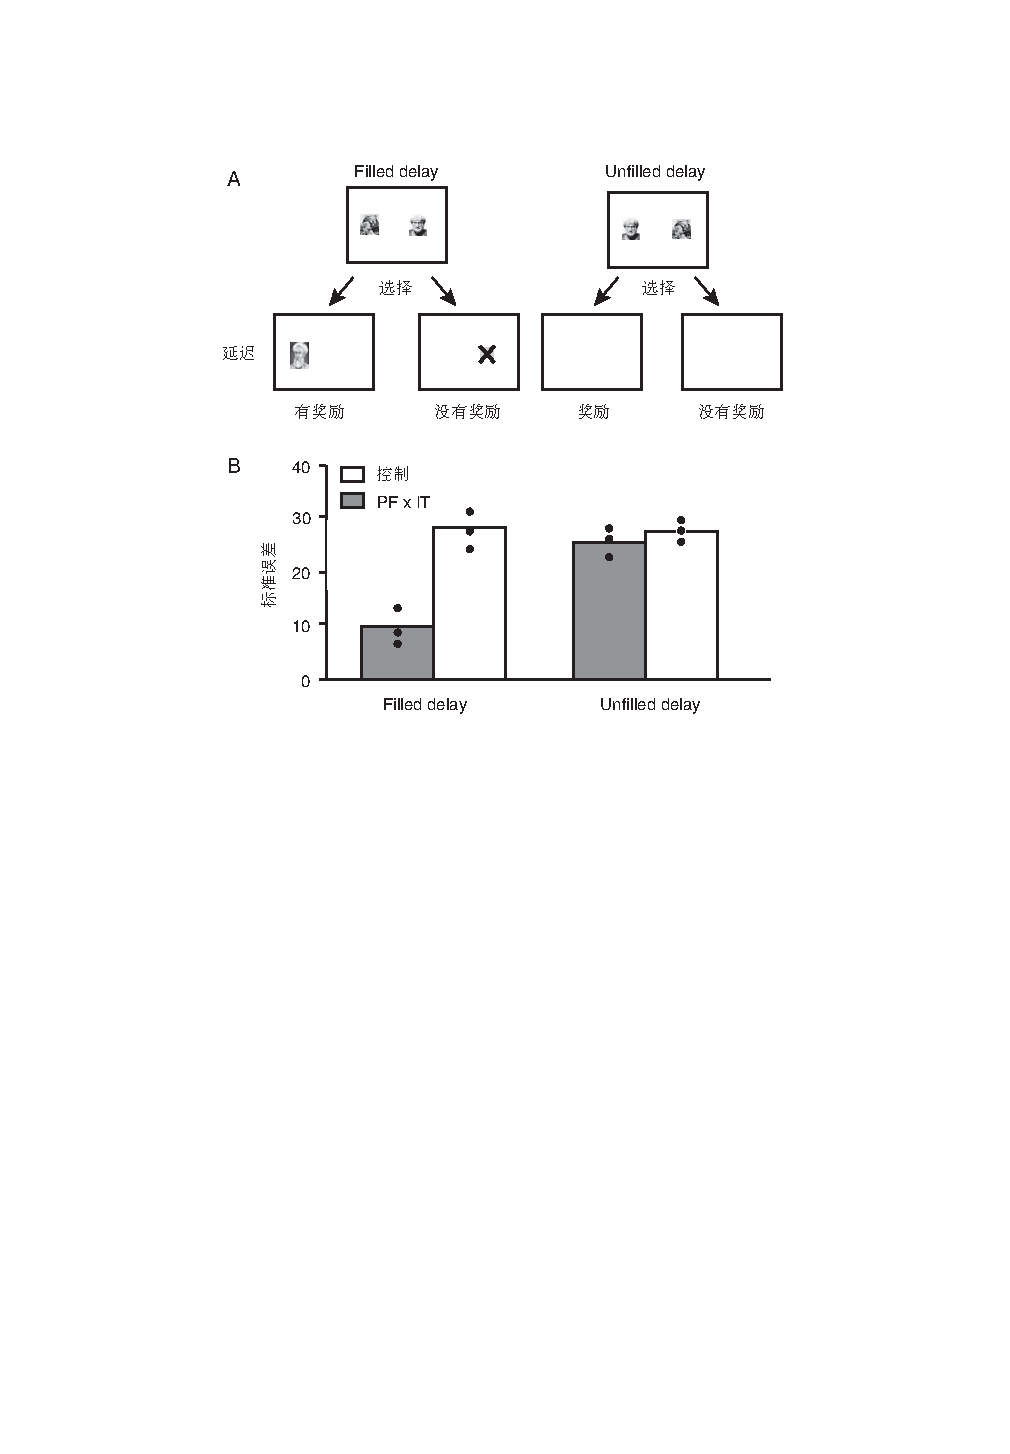
\includegraphics[width=0.7\linewidth]{chap8/fig_8_8}
	\caption{研究时间延长事件的任务中的事件。
		(A)上图表示猴子看到的屏幕。
		在猴子通过触摸其中一张图片做出选择后,如果猴子选择正确,则在获得奖励之前会有一个延迟期。
		在填充延迟条件下,延迟期间会出现刺激,该刺激与所选刺激特别相关。
		对于未填充延迟条件,延迟期间不会出现任何图片。
		(B)与正常(对照)猴子(白色条)相比,将前额叶皮层与下颞皮层 (PF × IT) 断开的效果(灰色条)。
		条形图显示组平均值,实心圆圈表示单个猴子的表现\cite{wilson2010functional}。 \label{fig:8_8}}
\end{figure}



\subsection{事件记忆与情景记忆}

在本章中,我们有意使用事件这个术语,而不是情景记忆。
首先,在我们提出的账户中,选择目标并不总是需要记忆。
有时候,猴子使用事件来立即选择未来的目标,就像在辨别学习任务中一样。
第二,情景记忆这个术语通常指的是比事件更具体的东西。
最初,情景记忆适用于与时间和空间背景相关的事件的外显回忆(Tulving 1983)。
我们承认,没有任何实验表明,猴子回忆事件的意义上重新体验的事件和他们的参与,因为人类做的(Suddendorf \& Busby 2003)。
然而,我们不需要提出这种主张。
可以说,一个事件是由特定时间和地点发生的背景、目标、行动和结果的结合构成的。
回想一下,在我们的术语中,术语目标指的是一个对象或一个地点,术语结果指的是成本和收益方面的反馈。
因此,一个事件,正如我们所使用的术语,考虑到选择的背景基础,选择作为行动目标的对象或地点,选择和做出的行动,以及该行动的结果。
前额叶皮层似乎通过与海马系统的连接(第~\ref{chap:chap3}~章)获得事件记忆,通过与感觉皮层的连接获得当前事件。
当前和记忆中的事件一起构成了我们所说的当前背景。



\subsection{总结}

我们建议,颗粒状前额叶皮层允许类人猿灵长类动物使用一个单一的事件,以改善选择。
通过依赖于这种能力的快速和抽象的学习,类人猿做出的风险或浪费的选择比其他情况下要少。
当病变或实验操作消除了这些优势时,类人猿灵长类的表现与其他哺乳动物更接近--可能也与它们的祖先相似。



\section{基于注意力控制生成目标}

在前面的两节中,我们已经将基于事件和当前上下文的目标生成与基于强化学习的行为进行了对比。
强化学习系统积累了许多过去经验的平均值,以调整指导行为的关联,例如行动-结果关联。
相比之下,灵长类动物选择目标的方式涉及使用单个事件选择物体和地点作为目标的能力,这种新的学习机制在快速变化的环境中提供了优势。
除了在资源异常波动的情况下,更古老、更慢的学习机制工作得很好,这解释了为什么几乎所有的动物王国都可以在没有颗粒状前额叶皮层的情况下茁壮成长。
但是,在早期灵长类历史的特定时间和地点,以及类人猿历史的特定时期(第 \ref{chap:chap2} 章),颗粒状前额叶皮层新区域的发育改善了它们的选择质量,从而提供了选择优势。
在本节中,我们将把灵长类动物选择目标的方式与注意力的概念联系起来,并将注意力控制行为与自动控制行为进行对比。
在我们的术语中,注意力提供了一种目标生成机制,与自动的目标的选择。
自动行为使动物能够将注意力集中在其他事情上,并且在行为的速度和可靠性方面提供了优势。
我们提出,旧的强化学习系统产生自动行为,而依赖于颗粒状前额叶皮层的新系统产生注意行为:
基于单一事件的行为和第 \ref{chap:chap6} 章和第 \ref{chap:chap7} 章描述的高级当前环境。
自动行为和注意行为之间的区别类似于自动行为和“控制”行为之间的区别,因为这些术语用于过程解离程序。
然而,我们要强调的是,当我们把注意力控制这个短语用在猴子身上时,我们并不意味着暗示任何关于意识的事情。
在实验室中,双重任务范式提供了自动性测试。
该程序测试次要任务的执行干扰主要任务的执行的程度。
例如,Baddeley\cite{shallice1996domain}表明,当人类受试者产生一系列随机数字时,如果同时他们必须执行记忆任务,则该系列变得更加刻板。
当然,不同的任务对注意处理的要求不同,但原则是一样的。
因此,一个主要任务的竞争任务的脆弱性提供了一个操作定义的专心控制的行为。
不知何故,主要任务“失去”控制行为的“比赛”,或者至少在某种程度上处于不利地位。
累加器网络提供了一种思考这种竞争的方法。
在第~\ref{chap:chap3}~章中,我们认为习惯可以战胜结果导向行为,因为与后者相比,前者依赖于更少和更强的关联。
因此,习惯网络可以更快地达到阈值,并“赢得”控制行为的竞争。
相反,注意控制的行为可能比自动行为依赖更多和更弱的关联。
因此,注意力行为网络达到阈值的速度比那些替代品和“失去”的竞争。
通过抑制依赖于较强联想的优势行为或通过增强注意力,较弱的联想可以占上风。
因此,注意力控制的行为与本书讨论的其他注意力形式类似。
第~\ref{chap:chap3}~章表明,前额叶皮层的部分产生的系统发育的老系统之间的偏见,竞争控制行为。
第~\ref{chap:chap5}~章回顾了一些证据,这些证据表明,前额叶皮层的某些部分会在皮层其他部分的相互竞争的感觉表征中产生偏见。
同样,我们认为前额叶皮层的部分区域会产生对目标生成网络的偏好,这些网络依赖于许多弱关联。
影像学研究支持注意控制和自动控制之间的区别。
例如,Toni等人\cite{toni1998time}教导了人类受试者运动序列,并绘制了受试者改善其表现时前额叶皮层激活的程度。
大约45分钟后,激活水平降低到接近基线水平。
Floyer-Lea\cite{floyer2004changing}在类似的任务中使用了双重任务范式,以表明该序列随着练习而自动化。
他们还发现,在这种情况下,前额叶皮层的激活明显减少。
这些发现表明,随着任务变得更加自动化,前额叶皮层变得不那么活跃。
我们并不是说,当一项任务变成自动化的时候,前额叶皮层就没有活动了。
例如,Rainer\cite{rainer2002timecourse}在猴子执行延迟匹配样本任务时,在前额叶皮层中记录。
在延迟的早期,他们发现对熟悉的物体几乎没有响应,但在延迟结束时,这种响应又出现了。
因此,在刚刚引用的成像研究中缺乏显著的激活可能反映了\textit{血氧水平依赖}信号的不敏感性。
尽管如此,成像结果显示了前额叶皮层神经处理的一些重要内容。
随着任务自动化,有些东西会减少。
而且,随着任务变得自动化,同时在几个区域的激活增加。
在运动任务中,这些结构包括壳核和小脑\cite{floyer2004changing,toni1998time}的报告。
在文献中,将自动行为等同于习惯并假设基底神经节有助于习惯已经变得普遍\cite{fernandez2001visual,broadbent2007rats}的报告。
直接证据表明,这种想法在两个方面都是错误的。
第一,自动行为比习惯更重要,这一点在第~\ref{chap:chap10}~章会讲到。
第二,只有一部分基底神经节维持习惯。
请注意,前面引用的成像结果是指壳核,而不是整个纹状体或基底神经节。
只有部分壳核被激活。
对大鼠的研究表明,纹状体中的不同区域在自动行为的不同方面起作用\cite{yin2008reward}。
纹状体的某些部分调节习惯,但其他部分调节结果导向行为,如第~\ref{chap:chap3}~章所定义的。
有些人声称,所有灵长类动物的行为,包括人类的行为,可以归类为习惯或结果导向的行为,他们将这两种行为分配给这两个纹状体区域\cite{balleine2010human}。
但比较证据表明,灵长类动物的纹状体中已经进化出了额外的区域,比如那些从颗粒状前额叶皮层接收输入的区域(第~\ref{chap:chap2}~章)。
下一节提出,基底神经节的这些新部分与颗粒状前额叶皮层一起发挥作用,以单个事件为基础产生目标。



前额叶-基底神经节环

神经生理学数据支持这一建议。
例如,Pasupathy\cite{pasupathy2005different}记录了当猴子解决新的条件性视觉运动问题时颗粒状前额叶皮层和尾状核头部的活动。
回想一下,尾状核的头部是颗粒状前额叶皮层的主要纹状体区域,而纹状体的更腹侧部分则从无颗粒前额叶皮层接收主要输入。
在Pasupathy等人的研究中,颗粒状前额叶皮层和尾状核头部的细胞在试验中随着学习的进展而逐渐提前编码目标。
活动的变化发生在纹状体比在皮层更快,虽然在整个试验的行为改善更接近观察到的前额叶皮层的变化较慢。
这些研究结果表明,颗粒状前额叶皮层和纹状体的领土成为从事在专注学习的视觉运动协会。
在条件性视觉运动学习期间,前运动皮层(区域6)投射到的纹状体区域中的细胞具有与运动前皮层中的细胞平行的与学习相关的活动变化\cite{brasted2004comparison}。
然而,在这些更尾部的地区,学习相关的活动的变化如下性能的改善,而不是之前,发生在颗粒状前额叶皮层的纹状体领土。
此外,活动的变化继续作为科目练习的运动,它的进展自动化。
这一证据表明,颗粒状前额叶皮层和纹状体领土调解注意的行为,而更多的尾侧皮层基底神经节回路调解自动行为。
最近的证据支持这一结论。
Antzoulatos\cite{antzoulatos2011differences}记录了颗粒状前额叶皮层及其纹状体区域中的神经元活动。
他们的猴子学会了将视觉类别映射到左或右目标的扫视眼球运动。
Antzoulatos和米勒首先证实了刚才提到的条件性视觉运动学习的发现。
当猴子能够学会将样本刺激映射到目标时,纹状体活动比皮层活动更早地编码目标。
然而,当猴子学会对每个类别中的许多样本进行分类时,编码类别到目标映射的皮层活动比纹状体活动更早发展。
因此,总的来说,颗粒状前额叶皮层和纹状体的领土功能,以支持注意,而不是自动的行为。
Miyachi等人\cite{miyachi1997differential}提供了进一步的证据来区分用于注意行为的吻侧纹状体系统和用于自动行为的更尾部纹状体系统。
他们教猴子一系列的动作,并对它们进行过度训练,直到这些动作成为自动动作。
然后,他们灭活了头侧纹状体或更多的尾侧部分。
喙失活包括头的尾状核和最喙的部分壳核,从颗粒状前额叶皮层接收输入。
更多的尾部失活包括壳核的部分,从初级运动皮层和运动前皮层接收输入。
Miyachi等人研究表明,失活的吻侧纹状体损害新的学习,而失活更多的尾部受损的自动性能。
此外,随着执行变得自动化,头侧纹状体中的活动减少,而中纹状体中的活动增加\cite{miyachi2002differential,brasted2004comparison}的研究结果一致。
因此,作为一个任务成为自动的转移发生从颗粒状前额叶皮层及其纹状体领土的自动控制由运动前皮层及其纹状体领土的注意控制。
为了测试运动前皮层和纹状体之间的连接是否在运动任务成为自动时必不可少,Nixon等人\cite{nixon2004cortico}教授猴子条件视觉运动任务,并对它们进行了3个月的过度训练。
这种行为就自然而然地发生了。
然后,作者通过在两个半球各做一个损伤,将纹状体与运动前皮层分离(图~\ref{fig:8_9}B)。
在一侧,他们损伤了苍白球,它通过丘脑将纹状体输出传递到运动前皮层。
另一边他们损伤了前运动皮层。这种结合损伤消除了对任务的所有记忆。
动物重新学习的时间和它们第一次学习的时间一样长(图~\ref{fig:8_9}A)。
因此,相对自动的行为控制依赖于运动前皮层和纹状体区域之间的相互作用。


\begin{figure} 
	\centering
	\includegraphics[width=0.7\linewidth]{chap8/fig_8_9}
	\caption{断开运动前皮层与基底神经节的连接对条件性视运动任务表现的影响。
		(A)白色条表示初始学习的错误次数,以及在测试中断后进行术前“重新学习”测试的错误次数。灰色条表示损伤后重新学习任务所需的试验次数(术后测试)。
		(B)损伤和相关连接的图示。
		灰色:每个半球的损伤结构和受影响的连接。
		黑色:每个半球的完整结构和连接。转载自 Nixon PD、McDonald KR、Gough PM、Alexander IH、Passingham RE。
		皮层-基底神经节通路对于回忆已建立的视运动关联至关重要\cite{nixon2004cortico}。 \label{fig:8_9}}
\end{figure}



前额叶-cerebellar循环

就像涉及纹状体和颗粒状前部皮层的回路一样,也有涉及小脑和颗粒状前部皮层的回路,特别是中外侧前部皮层\cite{kelly2003cerebellar}。
其他回路涉及小脑、前运动皮层和初级运动皮层\cite{strick2009cerebellum}。
我们已经提到,当运动序列任务变为自动时,小脑的激活会增加\cite{floyer2004changing}。
其中一些激活发生在齿状核,它通过丘脑投射回皮层。
为了观察小脑损伤是否会导致对前额叶皮层损伤敏感的任务受损,Nixon\cite{nixon1999cerebellum}在齿状核和间质核中进行了损伤。
猴子可以重新学习延迟的交替任务,而颗粒状前部皮层的损伤严重损害了交替任务。
在随后的一项研究中,有相同损伤的猴子可以学习新的动作序列。
然而,在响应时间的测量上,它们从未达到与正常动物相同的自动性水平\cite{nixon2000cerebellum}。
Lu等人\cite{lu1998role}也教猴子一些不同的动作序列,他们在其中的一个子集上对动物进行了过度训练。
在齿状核失活期间,猴子可以正常学习新的序列,但对于过度训练的自动序列,它们的眼手协调能力受损。
综上所述,这些发现支持小脑对自动行为计时的贡献。
为了支持这一观点,Ramnani\cite{ramnani2001changes}报告说,当受试者学习运动序列的时间直到它们成为自动的时候,小脑皮层的激活会增加。
这些变化发生在连接前部皮层的小脑小叶。
Nixon\cite{nixon2001predicting}发现,当目标发生在可预测的时间,而不是不可预测的时间时,齿状核和间质核受损的猴子在响应时间上没有表现出改善。
因此,小脑对自动行为控制的具体贡献可能涉及行动的时机,而不是行动的选择。



接合注意力控制

在资源稳定的环境中,依赖于先前事件的平均值,快速而自动地行动是值得的。
当这种行为不能产生一致的结果时,转向注意力控制是有意义的。
向注意控制模式的转换可能由奖励预测错误信号或第~\ref{chap:chap3}~章提到的其他有符号和无符号错误信号触发,这些信号可能来自几个来源中的任何一个,包括中脑多巴胺能细胞或杏仁核细胞。
Rowe等人\cite{rowe2002attention}利用人体成像技术研究了从自动控制到注意控制的转换。
他们的实验对象用四个手指做简单的动作。
以固定的顺序移动四个手指几乎不需要注意,在这种情况下,颗粒状前额叶皮层没有发生明显的激活\cite{rowe2002attention}。
但当受试者被指示注意他们的行为时,颗粒状前额叶皮层和\textit{前辅助运动区}发生了显著的激活。
Lau等人\cite{lau2004attention}报告说,当他们通过要求受试者报告他们第一次意识到自己要移动的意图的时间来操纵受试者的注意力时,同样的两个区域被激活。
总而言之,当人们注意自己的行为或意图时,激活发生在颗粒状前部皮层和前脑区,从而参与注意力控制。
在第~\ref{chap:chap9}~章中,当我们考虑人类前额叶皮层的额外层次时,我们再次讨论这些发现。



总结

本节强调,当一种行为成为自动行为时,由颗粒状前部皮层及其纹状体区域进行的注意控制将让位给由运动前皮层及其纹状体区域进行的自动控制。
有些人可能会问,颗粒状的前部皮层和纹状体区域在哪里。
从某种意义上说,它们位于涉及颗粒状前额皮层和前运动皮层的回路之间。
第~\ref{chap:chap3}~章回顾了颗粒状前部皮层偏向于调节习惯(S-R关联)和条件结果导向行为(R-O和S-R - o关联)的大脑结构的证据。
我们建议偏向于最适合当前行为背景的那种关联。
这个想法表明,前部皮层的颗粒部分,就像颗粒部分一样,在行为的集中控制中发挥作用。
但颗粒状区域与颗粒状区域的不同之处在于,它们是通过调节自动控制来实现的:这是强化学习系统的产物。
其功能可视为介于颗粒状前额叶 -基底神经节环和运动前基底神经节环之间。



\section{前脑皮层的基本功能}

在本章的这一点上,我们解释了颗粒状前部皮层的连接将其置于一个独特的位置:它位于上下文,目标和结果层次的顶端。
我们回顾了证据,表明它的功能是基于复杂的当前环境和单一事件产生目标。
因此,颗粒状的前部皮层减少了错误,并在专注的过程中加快了学习速度,而不是自动控制行为。
这种能力代表了行为控制的质变,从依赖于缓慢调整的刺激-响应-结果关联的系统发育上的旧机制到基于参与的一次性事件的新机制。
从最广泛的意义上说,颗粒状前部皮层赋予灵长类动物一种新的方式来知道在非常规情况下该做什么\cite{wise2008forward},而这些情况需要集中控制。
考虑到这一切,现在是时候提出颗粒状前部皮层的基本功能了,它比“知道在非常规情况下该做什么”更具特异性和更强的可测试性。
到目前为止,我们所说的取决于对这个问题采取自上而下的办法。
我们想看看我们的想法是否能解释现有的证据。
接下来,我们使用自下而上的方法,看看我们是否可以从观察中建立相同的想法。



行为和生理指纹

表8.1列出了一些有前额叶皮层病变的猴子表现不佳的任务。
正如第~\ref{chap:chap1}~章所解释的那样,它们共同构成了一种行为指纹。
该表还显示了各种任务所需的行为的一些组成部分。
表8.2列出了前额叶皮层神经元的一些特性。
它们共同构成了生理指纹。
为了允许对表进行引用,每个任务(T)和细胞活动类别(C)都有一个字母和数字标识。
例如,T1表示延迟响应任务(表8.1),C1表示回顾性延迟期活动(表8.2)。
我们从这些表格中看到了关于前额叶皮层功能的六个主题:整合、干扰、灵活性、前景、序列和估值。
毫无疑问,其他作者会列出不同的任务和额外的单元格属性。
他们可以强调不同的主题,如分类、抽象、集合、抑制、计划、监控和注意。
其中一些差异代表了真正的分歧,第~\ref{chap:chap10}~章讨论了一些关于前部皮层功能的不同观点。
有些只是代表术语上的差异:注意解决干扰;探矿包括设定和规划;分类是整合的结果。
1.集成。
表8.1中的许多任务依赖于前部皮层的整合功能,我们在前面的连词中讨论过。
条件任务(T6-8)依赖于上下文-目标-结果连词,对象就位场景任务(T19)需要使用背景来进行上下文连接,并且贬值任务(T22)要求将特定食物的外观、味道和当前价值结合起来。
许多种类的细胞活动也反映这样的连词(C5, C6, C28),如第~\ref{chap:chap6}~章所讨论的(见表6.1)。
2.干扰。
表8.1列出了几个任务的干扰,干扰的解决取决于干扰者对相关项目的注意力。
第~\ref{chap:chap6}~章解释了延迟响应(T1)和延迟交替(T2)任务,猴子在记忆中有一系列的位置。
然而,只有最近的位置提供了选择当前目标以获得预期结果的上下文。其他人的作用是分散注意力。
第~\ref{chap:chap6}~章对有序对象任务(通常称为自有序任务(T4))上的对象给出了类似的说明。
与这种需求相一致,前额叶皮层细胞编码顺序(C3)和顺序连词(见表6.1)。
3.灵活性。
表8.1列出了许多任务的灵活性。
条件任务(T6, T7)和策略任务(T9)要求猴子在不同的试验中改变目标。
有时条件变化不那么频繁,在试验块中,如在逆向任务中(T13, T20)。
逆转会引起奖励预测错误信号,而前皮层的细胞活动反映了这种错误(C31)。
细胞在逆转任务(C19)、条件任务(C5、C6)和策略任务(C9、C12)中反映目标的转变。
4. 勘察。
表8.1列出了许多任务的前瞻,前瞻编码,在我们使用这个术语的意义上,涉及作为目标的对象和地点的短期记忆。
如前所述,前瞻编码对辨别学习集和反转学习集有重要贡献。
在这些任务中,猴子使用事件来产生目标,前瞻编码在间隔时间内将这些目标维持在短期记忆中。
在延迟响应任务(T1)中,前瞻编码维持了延迟期间的目标记忆,并保护其不受先前试验选择目标的干扰。
前瞻性编码发生在试验内(C8, C10)和试验间(C10)延迟期。
5. 序列。
许多任务需要产生一系列目标的能力(T17),细胞活动在一系列目标中编码每个目标(C16)。
规划一系列次要目标(T16, T17)的能力涉及到为该系列的不同组成部分(C17)编码的细胞亚群,它们在各种各样的时间框架内发挥作用。
延迟交替任务(T2)也可以看作是涉及序列的任务,因为当前目标依赖于前一个目标。
6. 估值。
猴子通过处理奖励反馈来学习表8.1中的所有任务,因此评估涉及到所有目标选择。
例如,使规则成为当前规则(T15)的事实是,如果遵循它,它会导致有益的结果。
颗粒状前额叶皮层中的许多细胞(C22-30)显示出各种类型的与结果相关的活动,如第~\ref{chap:chap4}~章所述。



建议

我们的自底向上方法产生了主题列表,而我们的自顶向下方法解释了许多任务的结果。
然而,为了弄清灵长类动物前额皮层的基本功能,我们需要综合一切。
为了迎接这一挑战,我们提交了一份提案,首先是简短的形式,然后是稍微详细阐述的版本,然后是对术语和概念的说明。
这一建议代表了第~\ref{chap:chap3}-\ref{chap:chap7}~章所阐述的关于前额叶皮层各主要区域的建议的高潮。
简而言之:颗粒状前额叶皮层生成适合当前上下文和当前需求的目标,并且它可以基于单个事件来实现。
扩展:颗粒状前部皮层的基本功能,作为一个整体,是产生目标-作为行动目标的物体和地点-在当前环境和预期结果中是适当的,根据当前的生物需求进行评估。
与系统发育上较老的学习系统相比,它可以基于单个事件专心地学习。
因此,它提供了一种减少错误的机制,它通过两种方式做到这一点:通过快速学习,以及通过提供一种学习和应用抽象规则和策略的机制。
必要时,前脑皮层在前瞻记忆中保存目标和目标序列,直到可以尝试实现它们。
由于我们使用的许多术语在不同的研究领域具有不同的含义,因此我们添加了以下解释性注释:“当前环境”包括当前感官受体可用的刺激以及与产生当前目标相关的最近事件。
通过“产生目标”,我们排除了习惯性的、条件化的、自动的、显性的或常规的行为。
通过“当前需求”,我们指的是这样一个事实,即在消耗某种特定资源达到一定数量后,对该资源的生物需求、驱动力或动机会减少。
通过“目标”,我们指的是作为行动目标的对象或位置。
在这个意义上,我们把目标和结果区分开来。
通过“事件”,我们指的是在特定时间和地点的背景、目标、行动和结果的结合。
通过“基于单个事件生成目标”,我们将基于单个事件的目标选择与基于多个事件平均强化的缓慢学习区分开来。
通过“抽象规则”,我们指的是以“与样本匹配规则”为例的认知操作。抽象是指一个特定的任务操作适用于任何刺激项目,无论是新的还是熟悉的。
我们所说的“策略”是指对某些行为问题的部分解决方案,或者是对一个问题的两个或多个解决方案中的一个。
从抽象规则的意义上说,策略必然是抽象的。
所谓“前瞻记忆”,我们指的是在短期记忆中对目标的编码和维护。



后果

如果我们的建议是有道理的,那么灵长类动物前额皮层的基本功能一定有很多后果。
表8.3根据前面讨论过的信息层次(上下文、目标和结果)和主题(集成、解决干扰、灵活性、前景、序列和估值)对其中一些进行了总结。
以上下文层次结构和集成主题为例。
这张表表明,灵长类动物可以整合所有感官领域的信息,它们可以整合不同时间的事件,它们可以整合背景、事件、行动,并且输出。跨时间整合导致“跨时间偶然性”;跨事件的整合导致序列和“临时扩展事件”;跨感觉域的整合产生多模态特征连词;跨范例的集成导致了分类和抽象。
该表继续列出剩余的层次结构和功能主题。
当我们把这些综合起来看,灵长类动物前额叶皮层的基本功能似乎有一个重要的结果:那些不能产生最有利结果、浪费精力或增加被捕食风险的觅食选择的数量减少。
在实验室测试中,该功能在各种行为测试中导致更少的错误和更快的学习:
1. 如果有足够的经验,猴子可以在一次试验中学习视觉辨别(图~\ref{fig:8_2})、条件视觉运动映射(图~\ref{fig:8_5})和物体就位连词(图~\ref{fig:3_10}~和~\ref{fig:8_4})。
2. 他们可以利用自己在类似问题上的经验来学习和应用抽象的规则和策略。抽象的规则和策略适用于任何刺激材料,因此心理学家有时称之为能力转移\cite{warren1966reversal}。
这种迁移可以减少在学习样本之前的错误\cite{bussey2001role}。
3.他们可以在当前事件的基础上选择未来目标,并将这些目标保存在前瞻性记忆中,就像他们在学习设定任务时所做的那样\cite{murray2006prospective,wilson2008prefrontal}。
4. 他们可以将结果分配给对象中的单个选择\cite{walton2010separable}。
5. 他们可以把这些减少错误的机制结合起来,因为他们的颗粒状前部皮层是一个整体。



自适应的优点

刚才提到的实验室任务似乎与灵长类动物的日常觅食行为相距甚远。
但正如第~\ref{chap:chap2}~章所解释的那样,灵长类动物往往寿命较长,而类人猿往往依赖于不稳定的食物资源。
因此,类人猿可以通过使用单一或不频繁的事件来指导他们的觅食选择。
减少觅食错误的能力具有至关重要的优势。
生活有时是残酷的,成功的机会很少,而危险却很多。
在一个充满竞争对手和捕食者的多变环境中,即使是一个错误的后果也可能是严重的,甚至是致命的。
在第一章中,我们承诺不仅解释灵长类动物的前皮层做什么以及它是如何执行该功能的,而且还解释了其发展背后的选择因素。
为了实现这一目标,我们在觅食选择方面重新提出了我们的建议:
灵长类动物的颗粒状前部皮层进化为一种适应,以减少系统发育上较老的学习机制产生的非生产性、高风险或昂贵的觅食选择的数量。
这些较旧的机制依赖于基于强化的缓慢、累积的关联强化,在许多反馈事件中平均。灵长类动物进化的新机制带来了单一事件——环境、目标、行动和结果的结合——来影响觅食目标的选择。
关于这种新的前额叶机制的信息在很大程度上取决于灵长类动物进化出来的视觉进步。
请注意,我们并没有声称灵长类动物的颗粒状前部皮层赋予了从单一事件中学习或在此基础上选择目标的独特能力。
说灵长类动物能做某事并不意味着其他动物不能。
老鼠和许多其他动物一样,如果吃完后感到恶心,就再也不会吃新的食物,这种现象被称为味觉厌恶效应\cite{rozin1971specific}。
一些物种表现出印记:从一次观看事件中对个体的长期识别\cite{bateson1969development}。
我们认为,许多其他特殊目的的学习机制也已经发展起来,可以在其特定领域调解一次试验学习。
在第~\ref{chap:chap1}~章中,我们讨论了这样一个事实,即大鼠可以使用单一事件来拒绝放射状迷宫的一只手臂作为当前目标(Olton et al 1982):这是一种优势的“赢-转移”策略。
第~\ref{chap:chap3}~章解释了大鼠自发地执行非匹配位置任务,该任务利用了它们对单个先验事件的响应的优势行为。
我们知道,老鼠可以利用情境,比如迷宫地板的纹理,根据一次经历来记住一个可见物体及其位置(Eacott \& Easton 2010)。
我们接受这一切,甚至更多。
然而,我们所主张的是,灵长类动物减少错误的方式比这种专门的系统更普遍地适用于更广泛的觅食问题。
由此带来的优势可能看起来很微妙,但它可能对类人猿灵长类动物的成功至关重要。
早些时候,我们列出了六个主题,似乎出现在大量的文献关于前部皮层:整合,干扰,灵活性,前景,序列和估值。
我们现在可以提出这些能力是如何影响觅食选择的。
1. 集成。
灵长类动物可以整合所有感官领域的觅食信息来代表当前的环境。
第~\ref{chap:chap2}~章解释了现代类人猿的祖先如何适应白天的生活,并发展出一个最终支持三色视觉的中央凹。
同一章解释了灵长类动物的背侧和腹侧视觉流,包括新的后顶叶区和颞叶区,也在进化。
中央凹视觉使类人猿在很远的地方就能注意到树木的许多细微的方面,当距离足够近时,还能看到哪些动物、树叶和果实可能在那里。
前部皮层在整合来自背侧流和腹侧流的信息以及来自其他感觉模式的信息方面起着关键作用。
这些信息使灵长类动物能够更好地选择探索哪块资源,以及在一块区域内获得(或避免)什么物品,以及以什么顺序。
在遥远的脑区之间的选择最终涉及到导航,因此海马体的功能需要与前皮层的功能相结合(第~\ref{chap:chap3}~章)。
选择在一个小块中获取什么,最终涉及到由前运动皮层控制的手部运动,特别是在灵长类动物进化的视觉主导的参照系中,伸手和抓握。
这些行为通常涉及视觉和体感信息的整合。
操作、触诊和触觉的探索在很大程度上依赖于“触觉中央凹”的输入,这代表了灵长类动物的另一种创新(第~\ref{chap:chap2}~章)。
此外,它们的听觉系统检测灵长类动物或鸟类在特定地点觅食时发出的叫声和其他声音(第~\ref{chap:chap7}~章),并将这些信息与视觉相结合。
2. 干扰。
记忆的干扰对觅食的类人猿来说是一个特别的问题。
它们主要以水果、昆虫和树叶为食,它们以许多相似的东西为食。
这些其他物品中的大多数不能满足它们目前的生物需要。自上而下的注意力会使感官输入的处理和记忆偏向于那些与这些需求相关的信息。
正如第~\ref{chap:chap6}~章所说,背侧前部皮层似乎在减轻不相关事件的干扰方面起着关键作用,部分是基于它们的时间顺序。
第~\ref{chap:chap5}~章解释了尾侧前部皮层在调节自上而下对感觉环境相关特征的注意中的作用。
3.的灵活性。
在第~\ref{chap:chap2}~章中,我们指出了类人猿灵长类动物进化的证据,以利用挥发性资源,如水果和嫩叶。
在这种情况下,灵活一点是值得的。
类人猿灵长类动物可以灵活地行动,部分原因是如果它的第一个选择的行动没有达到它的目标并产生预期的结果,它可以在记忆中保持目标并转向另一个行动。
因此,类人猿前部皮层提供的一个关键进展涉及独立于实现该目标所需的行动的目标表征的产生、维持和长期存储。
在很大程度上,正是由于这个原因,将行动层次结构细化为目标层次结构才显得如此重要。
本章解释了颗粒状前部皮层对目标层次的重要性。
4. 勘察。
如果一个目标可以独立于实现的方式来表示,那么它也可以独立于实现的时间来表示。
前瞻编码可以在记忆中维持暂时的远距离目标,第~\ref{chap:chap6}~章和第~\ref{chap:chap7}~章分别讨论了背侧和腹侧前额叶皮层在这一功能中的作用。
5. 序列。
目标可以按顺序和层次结构组合。
第~\ref{chap:chap6}~章解释了当一个目标需要一系列行动或从属目标时,类人猿灵长类动物可以提前准备序列中的每个元素,并规定它们的顺序和时间。
最终目标可以在前瞻记忆中保持即使次级目标可能会改变。
第~\ref{chap:chap6}~章还提出了背侧前额叶皮层在制定有效的顺序目标策略中的关键作用。
由于大多数类人猿在社会群体中觅食,个体在一个斑块内激烈竞争资源,因此获得一组选定的水果或叶子的有效计划可能提供特别重要的优势。
6. 估值。
如果在进食过程中,动物对某种食物接近饱腹感,这将降低这种食物的主观价值和生产这种食物的树木的种类。
当生物需求或优先级以这种方式改变时,觅食目标也会改变。
第~\ref{chap:chap4}~章解释了颗粒眶额皮层在灵长类动物评估物体方面的进展。



总结

根据我们的建议,类人猿灵长类动物的颗粒状前部皮层为它们提供了一种新的能力:利用单一事件产生目标的能力。
由颗粒状前部皮层实现的学习系统因此增强了祖先的强化学习系统,该系统通过缓慢和累积的联想调整来学习。
当面对类人猿灵长类动物在进化过程中遇到的觅食问题时——其特征是依赖于被子植物树的特定产品而导致的一段时间的匮乏和消耗——祖先系统不可避免地产生了大量错误。
错误是危险的,而且代价高昂。
它们的新学习系统和祖先的学习系统都能减少错误并最大化奖励,但灵长类动物的前皮层做得更快,这提供了一个至关重要的适应优势。
尽管我们在新的和古老的学习系统之间进行了对比,但我们的建议并不意味着前脑皮层完全独立于后者运作。
第~\ref{chap:chap3}~章和第~\ref{chap:chap4}~章提出,前部皮层的颗粒部分在影响习惯和其他条件行为方面发挥关键作用。
我们关于觅食选择的建议也不应该被理解为暗示在社会选择中没有类似的作用。



\section{结论}

早期灵长类动物

我们认为,早期灵长类动物的颗粒状前部皮层提高了它们在细枝生态位中发现和评估物体的能力。
他们可以学习,基于单一的经验,在视觉项目中选择产生给定的结果(第~\ref{chap:chap4}~章),他们可以对他们的目标保持公开和隐蔽的注意力(第~\ref{chap:chap5}~章)。
颗粒状前额叶区域的发展伴随着对细枝生态位的一系列适应。
这种以后肢为主导的运动模式的转变为一种新的进食技术解放了双手。
立体视觉的进步开启了灵长类动物成为通常被称为“视觉动物”的过程。
早期灵长类动物也出现了新的后顶叶和下颞叶区域,以及利用顶叶输入来指导视觉坐标框架内的伸手和抓握运动的前运动区域(第~\ref{chap:chap2}~章)。
在这种情况下,尾侧前部皮层在克服细枝生态位中的杂波和干扰方面具有优势(第~\ref{chap:chap5}~章)。
同样,颗粒状前部皮层通过对比细枝生态位中各种物品的当前生物学价值,主要基于视觉和特定选择与特定结果的联系,提高了在物体之间进行选择的能力(第~\ref{chap:chap4}~章)。


类人猿

后来,在类人猿灵长类动物的进化过程中,随着这些动物体型的增加,觅食范围的扩大,并开始依赖丰富但易挥发的资源,如成熟的果实和未成熟的叶子,更多颗粒状的前额叶区域出现了。
它们白天在竞争激烈的环境中觅食,面临着严重的捕食威胁。
这样的生活安置了一个重视做出正确的觅食选择,避免低效和昂贵的选择,并在有限的经验基础上学会快速做出选择。
新的类人猿颗粒区包括背侧和腹侧前额叶皮层,也可能包括极侧前额叶皮层。
这些区域随着视觉的进步而进化,如中央凹视觉和三色视觉(第~\ref{chap:chap2}~章)。
它们的视觉进步使这些灵长类动物在分析视野内物体的位置、颜色、形状、纹理、光泽度和半透明性方面达到了一个新的复杂水平。
他们新的前额叶区域使他们能够基于单一事件产生一个目标或一系列目标。
为此,他们复杂的感知环境,包括使用的地方,时间,和秩序的视觉事件(第~\ref{chap:chap6}~章),视觉场景(第~\ref{chap:chap3}~章),从视觉和声学信号(第~\ref{chap:chap7}~章)。
这些领域允许类人猿进化学习,根据单一的经验,目标的视觉场景选择(图3.10和~\ref{fig:8_4}),这两个对象的选择作为一个目标(图8.2),和目标选择的任意符号(图~\ref{fig:8_5})。
根据这本书中提出的观点,类人猿灵长类动物的前额叶区域是一种特殊目的的适应,它克服了类人猿历史上特定时间和地点的特定问题。
这些区域减少了这些动物在白天长途觅食时可能犯的错误,目的是为了获得反复无常的资源。
然而,类人猿解决特定觅食问题的方式对后来灵长类动物的认知产生了深远的影响。
他们通过进化出一种新的通用学习系统来解决他们的特殊问题——周期性的资源匮乏和人员流失,这种系统超越了祖先系统的局限性。
祖先的通用学习系统缓慢地调整刺激、响应和结果之间的联系,产生了太多的错误。
类人猿的学习方式有三个关键方面。类人猿的前额叶皮层通过快速学习,通常基于单一经验,非常迅速地解决觅食问题。
灵长类动物的前皮层通过学习和应用抽象规则和策略,通过吸收类似情况的经验来解决新的觅食问题。
通过对行为的细心控制,类人猿灵长类动物在表现不佳时可以克服祖先的学习机制,因为它们在觅食危机中不可避免地会这样做。
我们得出结论,在灵长类历史的两个关键时期,颗粒状的前皮层为我们的祖先提供了一种微妙的适应优势,一种特别适合他们的生态位、问题和机会的优势。
这个边缘的微妙之处解释了为什么没有颗粒状前额叶区域的非灵长类哺乳动物可以很好地生存,就像有损伤的灵长类动物一样。
灵长类动物和其他哺乳动物一样,没有颗粒状的前部皮层,而是依靠祖先的学习机制。
本章主要基于对猴子的研究,提出了灵长类动物前额叶皮层的一个简单功能。
如此基本的功能似乎永远无法解释人们在执行复杂的认知任务时前额叶皮层的激活。
因此,下一章将讨论如何解释这些激活。









